% ============================================================
%  WanderMate -- Project 3 Task 2 Deliverable
%  Team 8 · S26CS6.401 Software Engineering
%  Architecture Framework (IEEE 42010 + Nygard ADRs)
% ============================================================
\documentclass[12pt, a4paper]{article}

% ── Packages ────────────────────────────────────────────────
\usepackage[a4paper, top=2.5cm, bottom=2.5cm,
            left=2.8cm, right=2.8cm, headheight=15pt]{geometry}
\usepackage[utf8]{inputenc}
\usepackage[T1]{fontenc}
\usepackage{xcolor}
\usepackage{titlesec}
\usepackage{titletoc}
\usepackage{fancyhdr}
\usepackage{graphicx}
\usepackage{booktabs}
\usepackage{longtable}
\usepackage{array}
\usepackage{tabularx}
\usepackage{multirow}
\usepackage{colortbl}
\usepackage{enumitem}
\usepackage{mdframed}
\usepackage{tcolorbox}
\usepackage{hyperref}
\usepackage{parskip}
\usepackage{setspace}
\usepackage{ragged2e}
\usepackage{amsmath}
\usepackage{float}

\tcbuselibrary{skins, breakable}

% ── Colour Palette (matching task1 formal style) ────────────
\definecolor{headingblack}{HTML}{1A1A1A}
\definecolor{rulegray}{HTML}{888888}
\definecolor{tableheaderbg}{HTML}{2C2C2C}
\definecolor{tablealtbg}{HTML}{F5F5F5}
\definecolor{notebg}{HTML}{F7F7F7}
\definecolor{noteborder}{HTML}{AAAAAA}
\definecolor{bodytext}{HTML}{1A1A1A}
\definecolor{captiontext}{HTML}{444444}
\definecolor{linkcolor}{HTML}{000000}
\definecolor{adrbg}{HTML}{F0F4F8}
\definecolor{adrborder}{HTML}{6B7280}
\definecolor{adrstatus}{HTML}{047857}

% ── Hyperref ────────────────────────────────────────────────
\hypersetup{
    colorlinks=false,
    hidelinks,
    pdftitle={Project 3 Task 2 -- Architecture Framework},
    bookmarksnumbered=true,
}

% ── Section Formatting ──────────────────────────────────────
\titleformat{\section}
  {\large\bfseries\color{headingblack}}
  {\thesection.}{0.6em}{}
  [\vspace{0.1em}\textcolor{rulegray}{\titlerule[0.4pt]}\vspace{0.2em}]

\titleformat{\subsection}
  {\normalsize\bfseries\color{headingblack}}
  {\thesubsection}{0.6em}{}

\titleformat{\subsubsection}
  {\normalsize\bfseries\itshape\color{headingblack}}
  {\thesubsubsection}{0.6em}{}

\titlespacing{\section}{0pt}{16pt}{6pt}
\titlespacing{\subsection}{0pt}{12pt}{4pt}
\titlespacing{\subsubsection}{0pt}{8pt}{3pt}

% ── Table Column Types ──────────────────────────────────────
\newcolumntype{L}[1]{>{\RaggedRight\arraybackslash}p{#1}}
\newcolumntype{C}[1]{>{\centering\arraybackslash}p{#1}}

% ── Note / Callout Box ──────────────────────────────────────
\tcbset{
  notebox/.style={
    enhanced,
    breakable,
    colback=notebg,
    colframe=noteborder,
    leftrule=2pt,
    toprule=0.3pt,
    bottomrule=0.3pt,
    rightrule=0.3pt,
    arc=0pt,
    boxsep=2pt,
    left=8pt, right=6pt, top=5pt, bottom=5pt,
    fontupper=\small\color{bodytext},
  }
}

% ── ADR Box ─────────────────────────────────────────────────
\tcbset{
  adrbox/.style={
    enhanced,
    breakable,
    colback=adrbg,
    colframe=adrborder,
    leftrule=3pt,
    toprule=0.5pt,
    bottomrule=0.5pt,
    rightrule=0.5pt,
    arc=2pt,
    boxsep=4pt,
    left=10pt, right=8pt, top=8pt, bottom=8pt,
    fontupper=\small\color{bodytext},
  }
}

% ── Paragraph / List spacing ────────────────────────────────
\setlist[itemize]{leftmargin=1.6em, itemsep=1pt,
                  parsep=0pt, topsep=3pt, label=\textendash}
\setlist[enumerate]{leftmargin=1.6em, itemsep=1pt, parsep=0pt, topsep=3pt}
\setlength{\parskip}{4pt}
\setlength{\parindent}{0pt}

% ── Convenience macros ──────────────────────────────────────
\newcommand{\thcell}[1]{\textcolor{white}{\textbf{\small #1}}}
\renewcommand{\arraystretch}{1.3}
\newcommand{\code}[1]{\texttt{\small #1}}
\newcommand{\adrstatus}[1]{\textcolor{adrstatus}{\textbf{#1}}}
\newcommand{\reqid}[1]{\textsc{\small #1}}

% ============================================================
\begin{document}

% ── Title Page ──────────────────────────────────────────────
\thispagestyle{empty}

\begin{center}
  {\LARGE\bfseries WanderMate: Social Mobile Travel Planner}\\[0.8em]
  {\large Task 2 }\\[0.4em]
  {\large Architecture Framework}\\[0.3em]
  {\normalsize IEEE 42010 Stakeholder Analysis \& Nygard Architecture Decision Records}
\end{center}

% ── Table of Contents ───────────────────────────────────────
\tableofcontents
\newpage

% ============================================================
\section{Introduction}
% ============================================================

WanderMate is a collaborative mobile travel planner built as a React~Native (Expo) frontend communicating with a Node.js/Express backend, backed by MongoDB for persistent storage and Firebase Realtime Database for real-time event propagation. The system integrates multiple external APIs --- Google Places, OpenRouteService (ORS), the Nominatim geocoding API, and a disabled Overpass adapter --- all proxied through a backend API Gateway that acts as a secret vault and central policy enforcement point.

This document presents the \textbf{Architecture Framework} for WanderMate, structured in two parts:

\begin{enumerate}
  \item \textbf{Stakeholder Identification (IEEE 42010)} --- Identifying stakeholders, cataloguing their concerns, and defining viewpoints and views that address those concerns, following the ISO/IEC/IEEE 42010:2022 standard for architecture description.
  \item \textbf{Architecture Decision Records (ADRs)} --- Documenting four major design decisions using the Nygard ADR template, with rationale grounded in the WanderMate codebase.
\end{enumerate}

\begin{tcolorbox}[notebox]
  \textbf{Notation.} Throughout this document, requirement identifiers (\reqid{NFR-06}, \reqid{FR-20}) refer to the requirements catalogue in the Task~1 deliverable. Code references use \code{monospace} font and point to files in the WanderMate repository.
\end{tcolorbox}

\begin{figure}[H]
\centering
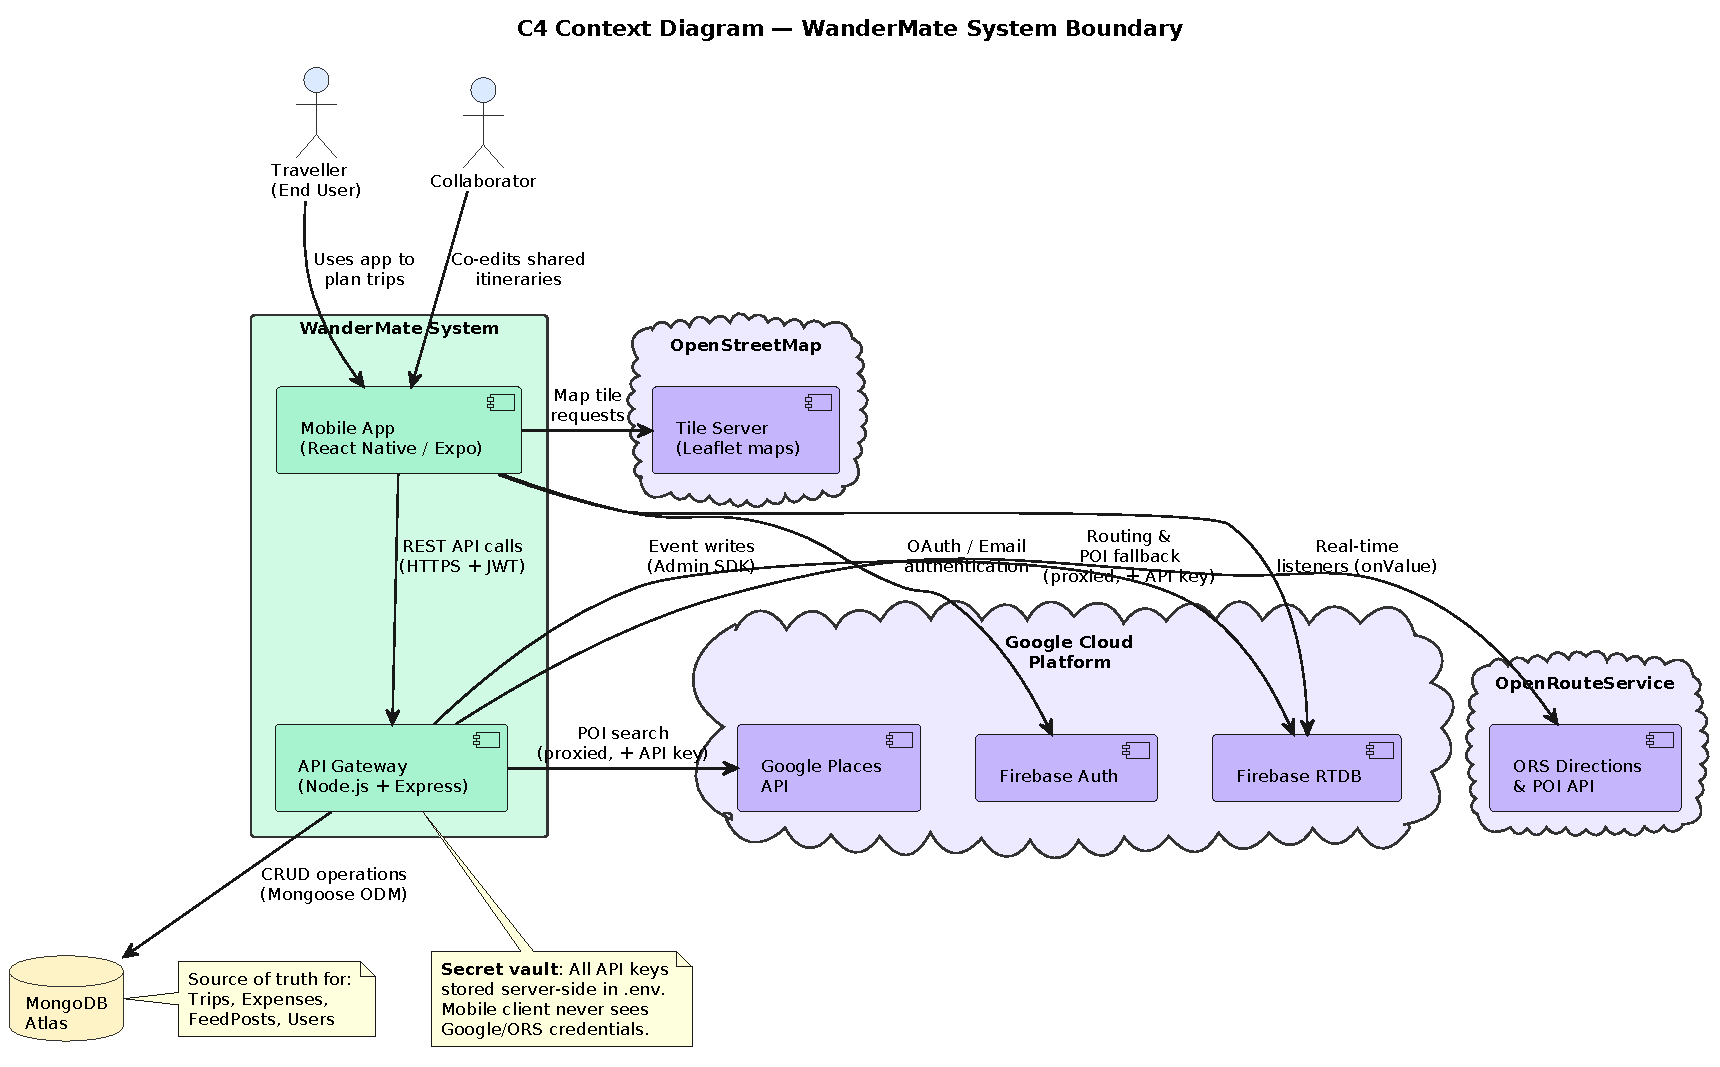
\includegraphics[width=0.95\textwidth]{c4_context.pdf}
\caption{C4 Context Diagram: WanderMate system boundary showing the two internal components (Mobile App, API Gateway), six external systems (Google Places, ORS, Nominatim, Firebase Auth, Firebase RTDB, MongoDB Atlas), and two actor types (Traveller, Collaborator). All external API credentials reside exclusively on the backend.}
\label{fig:c4-context}
\end{figure}

% ============================================================
\section{Stakeholder Identification (IEEE 42010)}
% ============================================================

ISO/IEC/IEEE 42010:2022 provides a conceptual framework for architecture description, centered on four core concepts: \textbf{stakeholders} who have \textbf{concerns} about the system, which are addressed by \textbf{viewpoints} (conventions for constructing a view) that produce \textbf{views} (concrete architecture work-products). This section applies these concepts to the WanderMate system.

% -----------------------------------------------------------
\subsection{Identified Stakeholders}
% -----------------------------------------------------------

The following stakeholders have been identified for the WanderMate system. Each stakeholder classification is derived from their role in the system's lifecycle and their interests in the architecture.

\begin{longtable}{C{0.5cm} L{2.8cm} L{4.0cm} L{6.0cm}}
\toprule
\rowcolor{tableheaderbg}
\thcell{\#} & \thcell{Stakeholder} & \thcell{Description} & \thcell{Representative Roles} \\
\midrule
\endhead
\bottomrule
\endfoot

1 & \textbf{End Users} (Travellers) & Individuals who use the mobile application to plan trips, discover POIs, manage budgets, and share itineraries. & Solo travellers, group trip organisers, travel enthusiasts browsing the social feed, collaborators on shared itineraries. \\

\rowcolor{tablealtbg}
2 & \textbf{Development Team} & Engineers responsible for building, testing, and evolving the WanderMate codebase across frontend and backend. & Frontend developers (React Native / Expo), backend developers (Node.js / Express), full-stack contributors. \\

3 & \textbf{Project Supervisor / Evaluators} & Academic supervisors and evaluation panels who assess WanderMate's architectural quality, adherence to requirements, and software engineering practices. & Course instructor, project evaluators, external reviewers. \\

\rowcolor{tablealtbg}
4 & \textbf{System Administrator / DevOps} & Individuals responsible for deploying, configuring, monitoring, and maintaining the backend infrastructure and database services. & Backend deployer, MongoDB Atlas administrator, Firebase console operator, environment configuration manager. \\

5 & \textbf{External API Providers} & Third-party services whose APIs WanderMate consumes, each with usage quotas, SLAs, and terms of service that constrain the system's architecture. & Google Cloud (Places API), OpenRouteService, Nominatim (OpenStreetMap), Firebase / Google Cloud Platform. \\

\end{longtable}

% -----------------------------------------------------------
\subsection{Stakeholder Concerns}
% -----------------------------------------------------------

Each stakeholder has specific concerns about the system. The table below exhaustively maps stakeholders to their primary concerns, with each concern traced to specific requirements from Task~1.

\begin{longtable}{C{0.5cm} L{2.5cm} L{5.8cm} L{3.8cm}}
\toprule
\rowcolor{tableheaderbg}
\thcell{ID} & \thcell{Concern} & \thcell{Detailed Description} & \thcell{Stakeholders \& Reqs} \\
\midrule
\endhead
\bottomrule
\endfoot

C1 & \textbf{Usability \& Responsiveness} & The mobile application must be intuitive, responsive, and provide quick access to core features (trip management, POI search, budgets, feed). UI interactions must feel native, with POI searches returning within 2 seconds and feed pages loading within 1.5 seconds. & End Users $\cdot$ \reqid{NFR-01}, \reqid{NFR-02}, \reqid{NFR-13} \\

\rowcolor{tablealtbg}
C2 & \textbf{Data Privacy \& Security} & User credentials and session data must be protected via industry-standard authentication (Firebase JWT). Third-party API keys must never be exposed in the mobile app bundle. Per-trip access control must be enforced server-side. & End Users, Sys.~Admin $\cdot$ \reqid{NFR-10}, \reqid{NFR-11}, \reqid{NFR-12} \\

C3 & \textbf{Offline Availability} & Users must be able to view and edit itineraries while offline (e.g., in airports, remote areas, underground transport). Mutations must be queued and synchronised upon reconnection without data loss. & End Users $\cdot$ \reqid{FR-03}, \reqid{NFR-07} \\

\rowcolor{tablealtbg}
C4 & \textbf{Modifiability \& Testability} & The codebase must be modular enough that adding or swapping an API provider (e.g., replacing Google Places with Mapbox) requires changes only in the relevant adapter, not in UI or routing layers. Each subsystem must be independently testable. & Dev Team, Supervisor $\cdot$ \reqid{NFR-14}, \reqid{NFR-15} \\

C5 & \textbf{Deployment \& Operations} & The system must be deployable with minimal configuration (environment variables in \code{.env}). Database connections, Firebase credentials, and API keys must be parameterised. The server must gracefully handle startup failures with clear error messages. & Sys.~Admin $\cdot$ \reqid{NFR-09} \\

\rowcolor{tablealtbg}
C6 & \textbf{API Quota Compliance} & The system must operate within the free-tier quotas of all external APIs at launch: Google Places ($\leq$ 5,000 req/month), ORS ($\leq$ 2,000 req/day), and Nominatim ($\leq$ 1 req/sec). Quota violations would incur financial cost and potentially break the service. & Supervisor, API Providers $\cdot$ \reqid{NFR-06} \\

C7 & \textbf{Real-time Collaboration} & Multiple users editing the same trip must see each other's changes propagated within 500\,ms. Conflict resolution must be automatic (without requiring user intervention), accepting that concurrent edits use a last-write-wins strategy which may silently discard intermediate changes. & End Users $\cdot$ \reqid{FR-20}, \reqid{FR-21}, \reqid{NFR-03} \\

\end{longtable}

% -----------------------------------------------------------
\subsection{Architecture Viewpoints}
% -----------------------------------------------------------

Following IEEE 42010, we define four viewpoints. Each viewpoint provides conventions for constructing and interpreting a specific kind of architecture view that addresses a subset of the stakeholder concerns.

\subsubsection{VP1: Functional Viewpoint}

\begin{tcolorbox}[notebox]
\textbf{Purpose:} Describes the system's runtime functional elements, their responsibilities, interfaces, and the interactions between them.\\[3pt]
\textbf{Concerns addressed:} C1 (Usability \& Responsiveness), C6 (Quota Compliance), C7 (Real-time Collaboration).\\[3pt]
\textbf{Stakeholders:} End Users, API Providers, Development Team.\\[3pt]
\textbf{Model kinds:} Component-and-connector diagrams, sequence diagrams.
\end{tcolorbox}

\textbf{View:} The functional structure of WanderMate is decomposed into six subsystems and one cross-cutting layer, as documented in Task~1 Section~4 (Subsystem Overview):

\begin{enumerate}
  \item \textbf{Mobile Client} (React Native / Expo) --- all user interaction, Zustand state management (\code{tripStore}, \code{budgetStore}, \code{feedStore}, \code{authStore}, \code{activeTripStore}), Leaflet WebView map, and offline cache (\code{localCache}, \code{syncQueue}).
  \item \textbf{API Gateway} (Node.js + Express) --- single backend entry point with middleware stack: \code{helmet()} security headers, \code{cors()}, \code{express.json()}, \code{generalLimiter} (100~req/15~min), and route-level \code{authenticate()} Firebase JWT verification (\code{middleware/auth.js}).
  \item \textbf{POI \& Routing Service} (\code{TravelService} Facade) --- encapsulates \code{PlacesAdapter} (Google Places), \code{ORSAdapter} (OpenRouteService), and the disabled \code{OverpassAdapter} behind a unified interface with \code{node-cache} caching (30~min search, 24~hr details, 1~hr routes). Also provides a \code{geocode()} method using Nominatim (OSM) with Google Places fallback for destination resolution. All search results are sorted by Haversine distance from the map centre and capped at 15 (text) or 20 (category).
  \item \textbf{Itinerary \& Budget Engine} --- \code{Trip} and \code{Expense} Mongoose models, trip/budget routes, \code{TripController} with owner/collaborator authorization checks, \code{TripObserver} event emitter for Firebase sync.
  \item \textbf{Social Feed \& Community Service} --- \code{FeedPost} model with denormalised snapshots, feed pagination (\code{skip/limit}), publish/like/clone endpoints, follower graph (\code{User.followers[]}/\code{following[]}).
  \item \textbf{Auth \& User Profile} --- Firebase Authentication (Email/Password + Google OAuth), \code{User} Mongoose model, \code{authStore} with \code{onAuthStateChanged} listener.
  \item \textbf{Real-time Sync Infrastructure} (cross-cutting) --- Firebase RTDB paths (\code{trips/\{tripId\}}, \code{budgets/\{tripId\}/lastUpdate}, \code{feed/\{postId\}}) with \code{onValue} listeners in frontend stores.
\end{enumerate}

The runtime interactions follow five primary data flows: POI \& Route Query, Collaborative Edit, Feed Publish, Itinerary Clone, and Offline Sync --- each documented with step-by-step sequence descriptions in Task~1 Section~5.

\subsubsection{VP2: Information Viewpoint}

\begin{tcolorbox}[notebox]
\textbf{Purpose:} Describes how information is stored, owned, managed, and accessed across the system. Defines the data ownership boundaries and consistency guarantees.\\[3pt]
\textbf{Concerns addressed:} C2 (Data Privacy \& Security), C3 (Offline Availability).\\[3pt]
\textbf{Stakeholders:} End Users, System Administrator, Development Team.\\[3pt]
\textbf{Model kinds:} Data model diagrams, data flow diagrams.
\end{tcolorbox}

\textbf{View:} WanderMate uses a \textbf{dual-database architecture}: MongoDB as the authoritative store for all domain data, and Firebase RTDB as a synchronization channel for real-time propagation.

\textbf{MongoDB data model} (Mongoose ODM):
\begin{itemize}
  \item \textbf{Trip} (\code{models/Trip.js}) --- nested document: \code{name}, \code{destination}, \code{startDate}, \code{endDate}, \code{owner} (Firebase UID), \code{collaborators[]} (UIDs), \code{days[]} $\rightarrow$ \code{stops[]} with \code{name}, \code{lat}, \code{lng}, \code{category} (enum of 13 types: hotel, restaurant, landmark, activity, transport, shopping, museum, park, nightlife, medical, grocery, finance, other), \code{order}, \code{cost}, etc. Indexes: \code{(owner, createdAt)}, \code{(collaborators)}, \code{(isPublished, publishedAt)}.
  \item \textbf{Expense} (\code{models/Expense.js}) --- separate collection, referenced by \code{trip} ObjectId. Fields: \code{user}, \code{description}, \code{amount}, \code{currency}, \code{category} (accommodation | food | transport | activities | other), \code{date}, \code{dayNumber}, \code{splitAmong[]}. Indexes: \code{(trip, date)} and \code{(trip, user)}.
  \item \textbf{FeedPost} (\code{models/FeedPost.js}) --- denormalised snapshot: \code{trip} (ref), \code{author} (UID), \code{authorName}, \code{tripName}, \code{destination}, \code{duration}, \code{totalBudget}, \code{stopCount}, \code{likes[]} (UIDs), \code{likeCount}. Indexes on \code{createdAt}, \code{(author, createdAt)}, \code{likeCount}.
  \item \textbf{User} (\code{models/User.js}) --- \code{firebaseUid} (unique), \code{email}, \code{displayName}, \code{avatarUrl}, \code{followers[]} (UIDs), \code{following[]} (UIDs), \code{publishedTrips[]} (ObjectId refs). Indexes on \code{firebaseUid} and \code{email}.
\end{itemize}

\textbf{Firebase RTDB paths} (sync layer):
\begin{itemize}
  \item \code{trips/\{tripId\}} --- carries a Firebase-safe snapshot of the full trip document on updates (including \code{updatedAt} and \code{lastEditedBy}). Written by \code{TripObserver} event handlers (\code{services/tripObserver.js}).
  \item \code{budgets/\{tripId\}/lastUpdate} --- timestamp written on expense mutations.
  \item \code{feed/\{postId\}} --- carries \code{\{author, tripName, createdAt\}} on publish.
\end{itemize}

\textbf{Data ownership and consistency:}
\begin{itemize}
  \item MongoDB is the \emph{single source of truth} for all complex queries and all writes (follower graphs, expense aggregations, feed pagination, trip mutations).
  \item Firebase RTDB is used as a synchronization channel: budget/feed paths carry lightweight notifications, while the trip path carries a server-produced trip snapshot for collaborator update propagation.
  \item The \code{TripObserver} (\code{services/tripObserver.js}) uses Node.js \code{EventEmitter} to decouple business logic from Firebase writes. The \code{TripController} emits events (\code{TRIP\_CREATED}, \code{TRIP\_UPDATED}, \code{TRIP\_DELETED}, \code{COLLABORATORS\_UPDATED}); the observer handles Firebase propagation.
  \item Client-side \code{localCache} (AsyncStorage) provides offline reads with infinite TTL; the \code{syncQueue} queues write operations for replay on reconnect.
\end{itemize}

\begin{figure}[H]
\centering
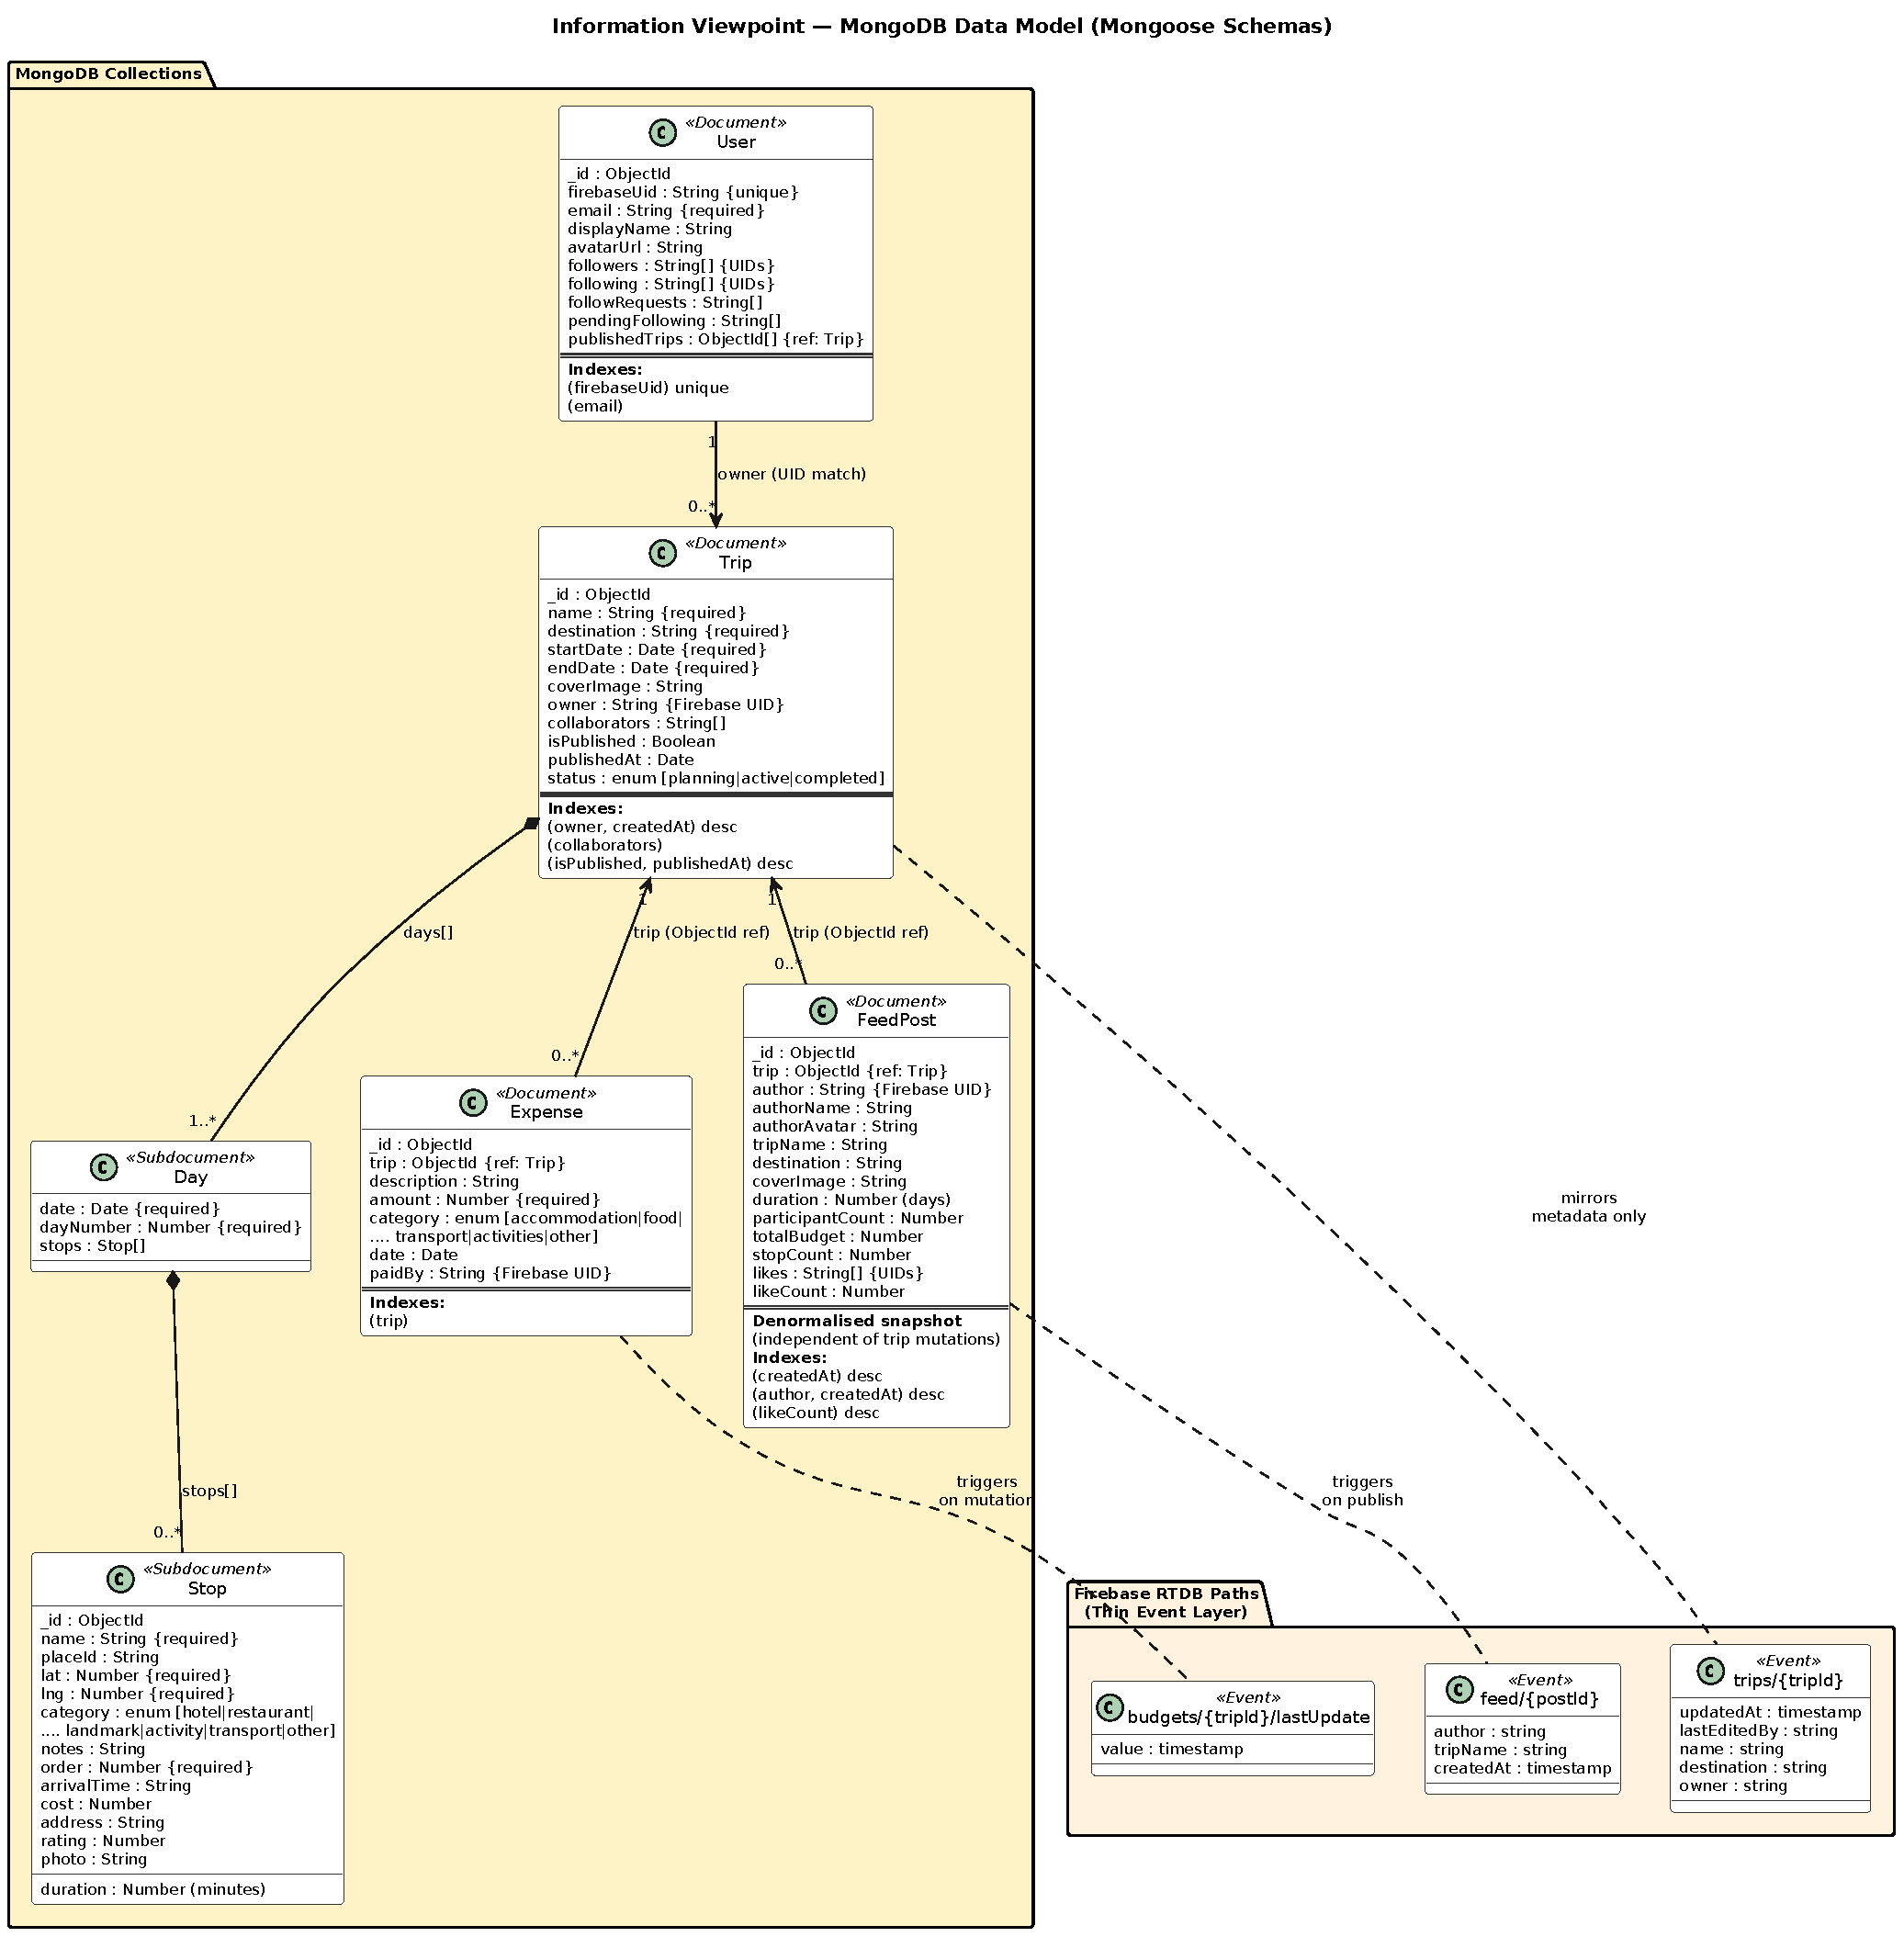
\includegraphics[width=\textwidth]{data_model.pdf}
\caption{Information Viewpoint --- MongoDB data model (Mongoose schemas) and Firebase RTDB sync paths. The four MongoDB collections (Trip, Expense, FeedPost, User) serve as the authoritative data store; Firebase paths are used for real-time propagation (trip snapshot sync plus budget/feed notifications).}
\label{fig:data-model}
\end{figure}

\subsubsection{VP3: Deployment Viewpoint}

\begin{tcolorbox}[notebox]
\textbf{Purpose:} Describes the mapping of software artifacts to the physical and cloud infrastructure, including network topology, service dependencies, and configuration management.\\[3pt]
\textbf{Concerns addressed:} C5 (Deployment \& Operations).\\[3pt]
\textbf{Stakeholders:} System Administrator, Development Team.\\[3pt]
\textbf{Model kinds:} Deployment diagrams, infrastructure topology.
\end{tcolorbox}

\textbf{View:} WanderMate is deployed as a two-tier architecture with three managed cloud services:

\begin{longtable}{L{3.0cm} L{3.5cm} L{6.5cm}}
\toprule
\rowcolor{tableheaderbg}
\thcell{Component} & \thcell{Runtime Target} & \thcell{Configuration \& Notes} \\
\midrule
\endhead
\bottomrule
\endfoot

Mobile Client & Android device / Expo Go & Built with Expo SDK 54 (managed workflow). Uses Expo Router for file-based navigation. API base URL configured via \code{frontend/config/env.ts} (\code{API\_BASE\_URL}). \\

\rowcolor{tablealtbg}
API Gateway & Node.js process (single instance) & Entry point: \code{backend/src/index.js}. Listens on port 5000. All secrets loaded from \code{backend/.env}: \code{MONGODB\_URI}, \code{FIREBASE\_*} credentials, \code{GOOGLE\_PLACES\_API\_KEY}, \code{ORS\_API\_KEY}. Dev mode: \code{node --watch src/index.js}. \\

MongoDB & MongoDB Atlas (cloud) & Connection via \code{MONGODB\_URI} in \code{.env}. Configured in \code{config/database.js} with Mongoose ODM (v9.4.1). Indexes pre-defined in model schemas for query performance. \\

\rowcolor{tablealtbg}
Firebase RTDB & Google Cloud (managed) & Configured via \code{FIREBASE\_DATABASE\_URL}. Backend uses Firebase Admin SDK (singleton in \code{config/firebase.js}). Frontend uses Firebase JS SDK (singleton in \code{config/firebase.ts}) with AsyncStorage auth persistence. \\

Firebase Auth & Google Cloud (managed) & Providers: Email/Password, Google Sign-In (OAuth 2.0 via \code{expo-auth-session}). Web client ID configured in \code{frontend/config/env.ts}. \\

\end{longtable}

\begin{figure}[H]
\centering
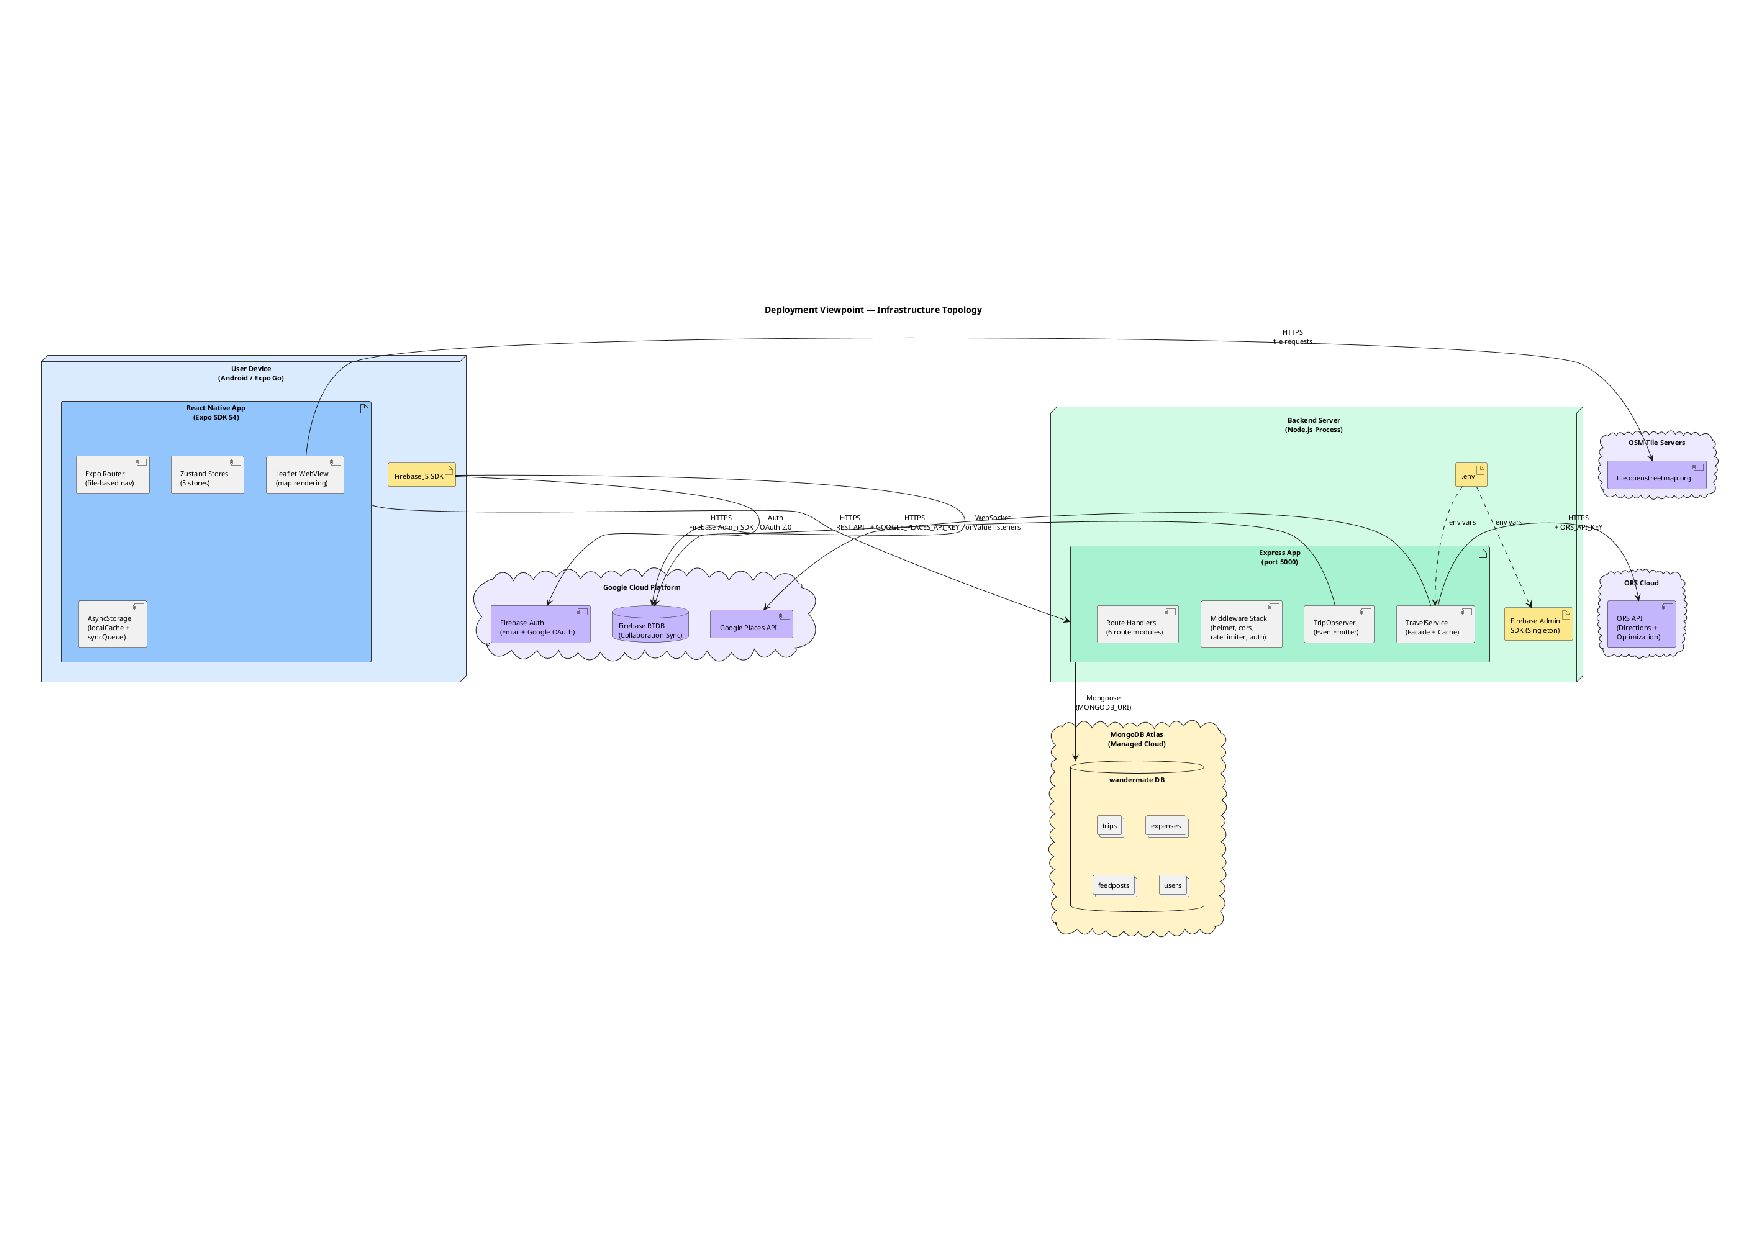
\includegraphics[width=\textwidth]{deployment_diagram.pdf}
\caption{Deployment Viewpoint --- infrastructure topology showing the User Device (React Native app with AsyncStorage), Backend Server (Express + middleware + TravelService), MongoDB Atlas, Firebase services, and external API providers. All connections labelled with protocol and credential flow.}
\label{fig:deployment}
\end{figure}

\subsubsection{VP4: Development Viewpoint}

\begin{tcolorbox}[notebox]
\textbf{Purpose:} Describes the organisation of the codebase into modules, packages, and layers to support the team's development, testing, and evolution workflow.\\[3pt]
\textbf{Concerns addressed:} C4 (Modifiability \& Testability).\\[3pt]
\textbf{Stakeholders:} Development Team, Project Supervisor.\\[3pt]
\textbf{Model kinds:} Package diagrams, layer diagrams, module decomposition.
\end{tcolorbox}

\textbf{View:} The WanderMate codebase follows a \textbf{four-layer architecture} on both frontend and backend, with strict downward dependency flow:

\textbf{Backend layers:}
\begin{enumerate}
  \item \textbf{Presentation} --- Express route handlers (\code{routes/trips.js}, \code{routes/poi.js}, \code{routes/budget.js}, \code{routes/feed.js}, \code{routes/users.js}, \code{routes/routes.js}) and the \code{TripController} class.
  \item \textbf{Business Logic} --- \code{TravelService} Facade (\code{services/travelService.js}), \code{TripObserver} EventEmitter (\code{services/tripObserver.js}).
  \item \textbf{Data Access} --- Mongoose models (\code{models/Trip.js}, \code{models/Expense.js}, \code{models/FeedPost.js}, \code{models/User.js}).
  \item \textbf{Infrastructure} --- Config files (\code{config/database.js}, \code{config/firebase.js}), middleware (\code{middleware/auth.js}, \code{middleware/cache.js}, \code{middleware/rateLimiter.js}).
\end{enumerate}

\textbf{Frontend layers:}
\begin{enumerate}
  \item \textbf{View} --- Expo Router screens (\code{app/(tabs)/}, \code{app/(auth)/}, \code{app/trip/}), reusable components (\code{components/}).
  \item \textbf{State Management} --- Zustand stores (\code{stores/tripStore.ts}, \code{stores/budgetStore.ts}, \code{stores/feedStore.ts}, \code{stores/authStore.ts}, \code{stores/activeTripStore.ts}).
  \item \textbf{Service} --- API client (\code{services/api.ts} with Axios interceptor for JWT injection), sync queue and local cache (\code{services/syncQueue.ts}).
  \item \textbf{Infrastructure} --- Firebase SDK init (\code{config/firebase.ts}), environment config (\code{config/env.ts}).
\end{enumerate}

This layered structure ensures that replacing a data provider (e.g., swapping Google Places for Mapbox) requires changes only in layer 2 (a new adapter in \code{services/}) and the \code{TravelService} constructor --- no changes to routes, stores, or UI screens. This was empirically validated when the \code{OverpassAdapter} was disabled: the change was confined to commenting out the import in \code{travelService.js} (NFR-15 compliance).

% -----------------------------------------------------------
\subsection{Stakeholder--Concern--Viewpoint Traceability}
% -----------------------------------------------------------

The following matrix provides full traceability from stakeholders through concerns to the viewpoints that address them:

\begin{longtable}{L{3.0cm} L{3.5cm} L{3.5cm} C{3.0cm}}
\toprule
\rowcolor{tableheaderbg}
\thcell{Stakeholder} & \thcell{Primary Concerns} & \thcell{Addressed by Viewpoints} & \thcell{NFRs Traced} \\
\midrule
\endhead
\bottomrule
\endfoot

End Users & C1 (Usability), C3 (Offline), C7 (Real-time Collab.) & VP1 (Functional), VP2 (Information) & NFR-01, NFR-07, NFR-03 \\

\rowcolor{tablealtbg}
Development Team & C4 (Modifiability \& Testability) & VP4 (Development), VP1 (Functional) & NFR-14, NFR-15 \\

Project Supervisor & C4 (Modifiability), C6 (Quota Compliance) & VP4 (Development), VP1 (Functional) & NFR-06, NFR-14 \\

\rowcolor{tablealtbg}
System Administrator & C2 (Security), C5 (Deployment) & VP2 (Information), VP3 (Deployment) & NFR-10, NFR-11 \\

API Providers & C6 (Quota Compliance) & VP1 (Functional) & NFR-06 \\

\end{longtable}

\begin{figure}[H]
\centering
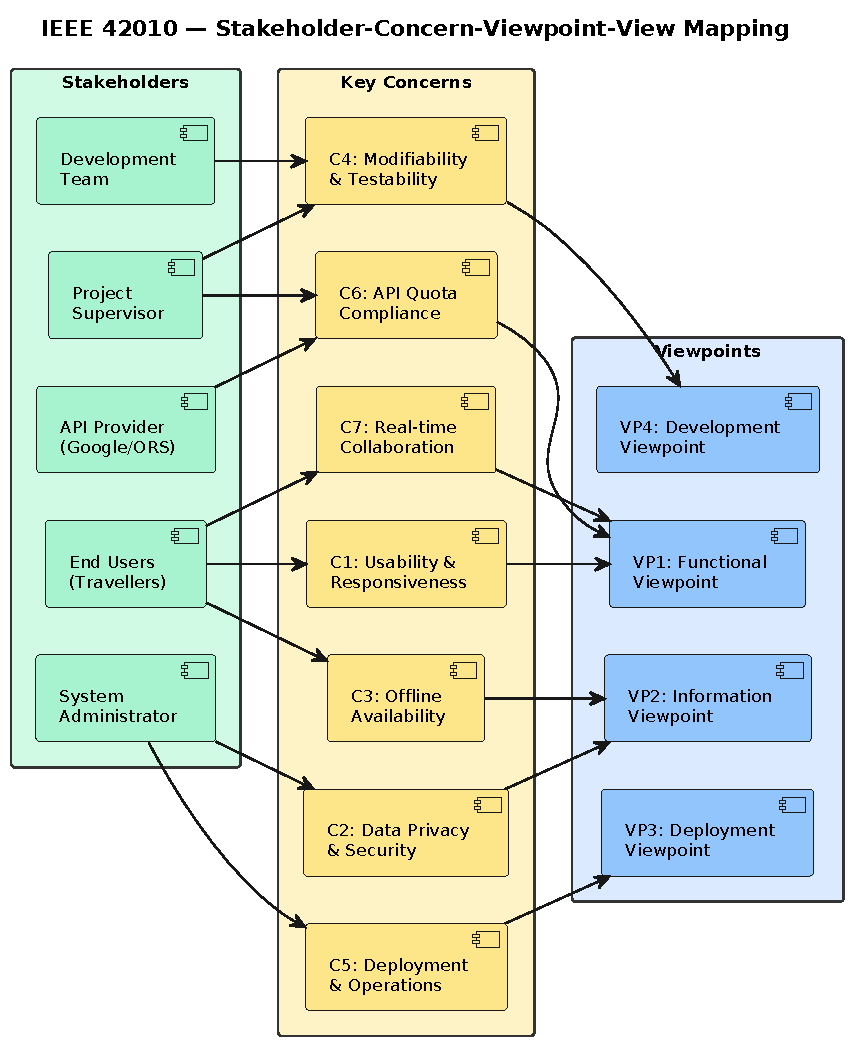
\includegraphics[width=\textwidth]{stakeholder_viewpoint.pdf}
\caption{IEEE 42010 traceability: stakeholders $\to$ concerns $\to$ viewpoints. Each arrow indicates that a concern raised by a stakeholder is addressed by the corresponding viewpoint.}
\label{fig:stakeholder-viewpoint}
\end{figure}

% ============================================================
\section{Architecture Decision Records (ADRs)}
% ============================================================

The following Architecture Decision Records document major design decisions using the \textbf{Nygard ADR template} (Title, Context, Decision, Status, Consequences). Each ADR is grounded in specific code artefacts and requirements from the WanderMate repository.

% -----------------------------------------------------------
\subsection{ADR-001: Use Firebase Realtime Database as a Collaboration Sync Channel (Not as a Primary Data Store)}
% -----------------------------------------------------------

\begin{tcolorbox}[adrbox]

\textbf{\large ADR-001: Use Firebase RTDB as a Collaboration Sync Channel}

\vspace{0.6em}
\textbf{Context}

WanderMate requires real-time collaborative editing: when one user modifies a shared itinerary, all connected collaborators must see the change within 500\,ms (\reqid{NFR-03}). At the same time, the system needs to support complex queries that Firebase RTDB is not optimised for:

\begin{itemize}
  \item Paginated feed queries sorted by \code{createdAt} with follower-based filtering (\code{FeedPost.find(\{author: \{\$in: following\}\}).sort(\{createdAt: -1\}).skip(skip).limit(limit)} in \code{routes/feed.js}, line~24).
  \item Per-trip expense aggregations with category breakdowns (server-side budget summary computation in \code{routes/budget.js}).
  \item Follower graph queries using adjacency-list relationships (\code{User.followers[]}, \code{User.following[]}).
  \item Cross-collection joins between \code{Trip}, \code{Expense}, and \code{User} documents during itinerary clone (\code{routes/feed.js}, lines~148--208).
\end{itemize}

We evaluated two architectural approaches:
\begin{enumerate}
  \item \textbf{Firebase-primary:} Use Firebase RTDB as the primary data store for all trip data, with real-time listeners providing both persistence and collaboration.
  \item \textbf{MongoDB-primary + Firebase-events:} Use MongoDB as the authoritative store for domain data, with Firebase serving only as a notification layer to trigger client re-fetches.
\end{enumerate}

\vspace{0.6em}
\textbf{Decision}

We will use \textbf{MongoDB as the single source of truth} for all domain data and \textbf{Firebase RTDB as a collaboration synchronization channel}. Trip writes are persisted to MongoDB first, then propagated to Firebase for real-time client updates.

Concretely:
\begin{itemize}
  \item Backend route handlers persist all mutations to MongoDB via Mongoose models, then emit events on the \code{TripObserver} EventEmitter (\code{services/tripObserver.js}).
  \item The \code{TripObserver} writes synchronization payloads to Firebase paths:
    \begin{itemize}
      \item \code{trips/\{tripId\}} $\gets$ full Firebase-safe trip snapshot on updates (including \code{updatedAt} and \code{lastEditedBy})
      \item \code{budgets/\{tripId\}/lastUpdate} $\gets$ timestamp
      \item \code{feed/\{postId\}} $\gets$ \code{\{author, tripName, createdAt: Date.now()\}}
    \end{itemize}
  \item Frontend stores subscribe via \code{onValue} listeners (\code{tripStore.subscribeTripUpdates()}, \code{budgetStore.subscribeBudgetUpdates()}). For trip updates, \code{tripStore} applies the Firebase snapshot directly when its \code{updatedAt} is newer (last-write-wins).
\end{itemize}

\vspace{0.6em}
\textbf{Status:} \adrstatus{Accepted}

\vspace{0.6em}
\textbf{Consequences}

\textbf{Positive:}
\begin{itemize}
  \item MongoDB remains the single source of truth, avoiding dual-write consistency issues.
  \item Complex queries (pagination, aggregations, graph traversals) are handled by MongoDB's query planner with proper indexes, not by Firebase's limited query model.
  \item Clients receive trip updates without requiring an additional API re-fetch round trip.
  \item The \code{TripObserver} EventEmitter (\code{services/tripObserver.js}) decouples business logic from sync infrastructure --- route handlers call \code{tripEvents.emit('TRIP\_UPDATED', trip.\_id, req.user.uid)} (e.g., \code{tripController.js}, line~104) without knowing about Firebase at all.
\end{itemize}

\textbf{Negative:}
\begin{itemize}
  \item Writing full trip snapshots to Firebase on each update increases RTDB write payload size compared with metadata-only notifications.
  \item Two infrastructure dependencies (MongoDB + Firebase) instead of one; both must be operational for full functionality.
  \item Conflict resolution relies on last-write-wins timestamps (\code{updatedAt}) rather than Firebase's built-in conflict resolution; complex concurrent edits may lose intermediate states.
\end{itemize}

\end{tcolorbox}

\begin{figure}[H]
\centering
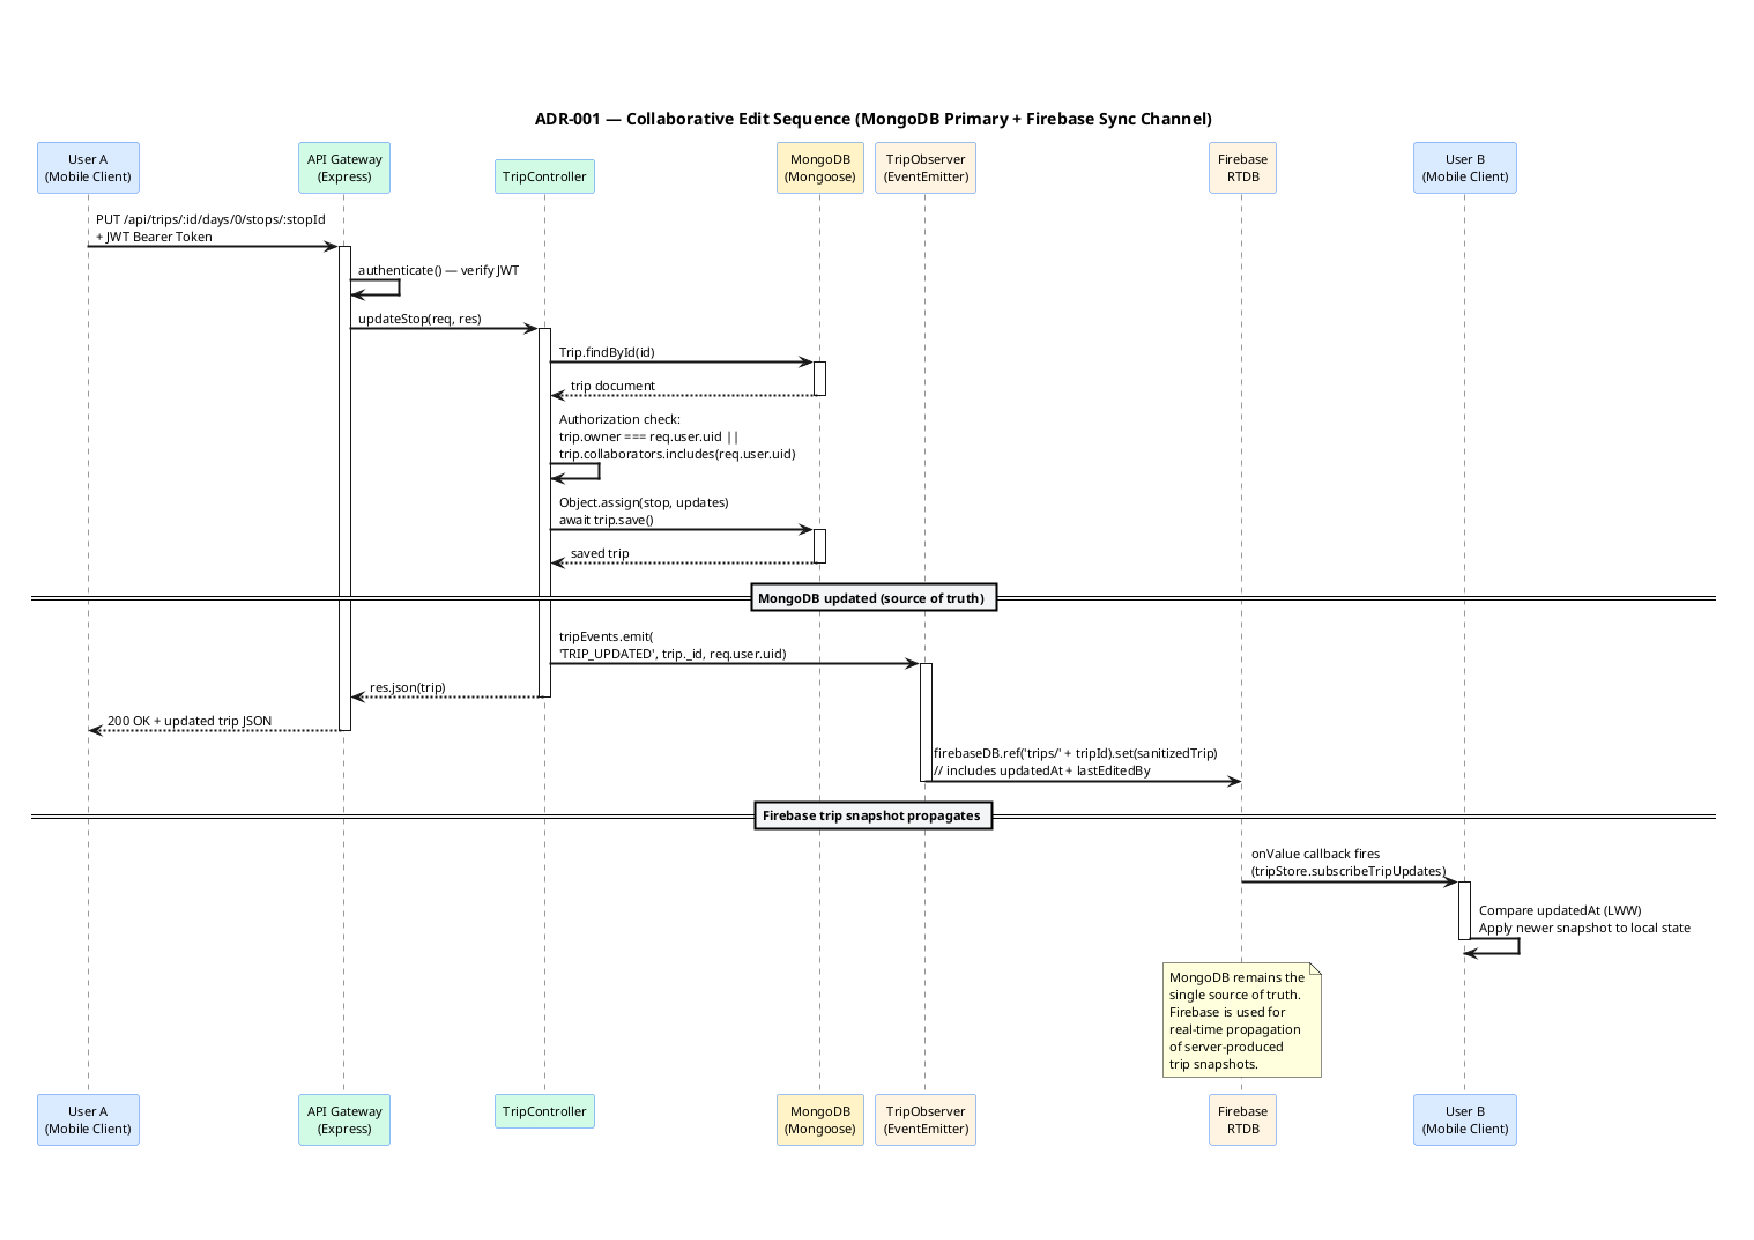
\includegraphics[width=\textwidth]{adr001_event_flow.pdf}
\caption{ADR-001 Sequence Diagram: collaborative edit flow. User~A mutates a stop via the API Gateway, which persists to MongoDB (source of truth), then emits a \code{TRIP\_UPDATED} event via \code{TripObserver}. The observer writes a Firebase-safe trip snapshot to Firebase RTDB. User~B's \code{tripStore} receives the \code{onValue} callback and applies the newer snapshot using last-write-wins checks.}
\label{fig:adr001-sequence}
\end{figure}

% -----------------------------------------------------------
\subsection{ADR-002: Adopt the API Gateway Pattern with Server-side Secret Proxying}
% -----------------------------------------------------------

\begin{tcolorbox}[adrbox]

\textbf{\large ADR-002: Backend API Gateway as Secret Vault and Policy Enforcement Point}

\vspace{0.6em}
\textbf{Context}

WanderMate consumes multiple external APIs, including those with sensitive credentials or strict SLAs:
\begin{itemize}
  \item \textbf{Google Places API} --- requires a \code{GOOGLE\_PLACES\_API\_KEY} with billing enabled. If extracted from a mobile bundle, it could be used by attackers to make arbitrary calls, incurring cost.
  \item \textbf{OpenRouteService API} --- requires an \code{ORS\_API\_KEY} with a daily quota of 2,000 requests.
  \item \textbf{Nominatim Geocoding API} --- strictly limits requests to 1 per second and requires a valid User-Agent, risking permanent IP bans if called freely from clients.
  \item \textbf{Firebase Admin SDK} --- requires a private key (\code{FIREBASE\_PRIVATE\_KEY}) that grants unrestricted access to the Firebase project (database administration, user management, custom token generation).
\end{itemize}

React Native applications are compiled into JavaScript bundles that can be extracted and decompiled from APK/IPA files using tools like \code{apktool} or \code{jadx}. Any API key embedded in the client-side bundle is, for practical purposes, a public key.

\reqid{NFR-11} explicitly requires: ``Third-party API keys shall never be embedded in the mobile app bundle.''

Two approaches were considered:
\begin{enumerate}
  \item \textbf{Direct client-to-API calls:} The mobile client calls external APIs directly, embedding keys in the bundle or fetching them at runtime from a config endpoint.
  \item \textbf{Backend proxy:} A server-side API Gateway proxies all external API calls, storing keys as environment variables that never leave the server process.
\end{enumerate}

\vspace{0.6em}
\textbf{Decision}

We will implement a \textbf{Node.js/Express API Gateway} (\code{backend/src/index.js}) that:
\begin{enumerate}
  \item Loads all API keys from \code{.env} via \code{dotenv} (line~1: \code{require('dotenv').config()}).
  \item Applies a middleware stack on every request:
    \begin{itemize}
      \item \code{helmet()} --- sets security headers (\code{X-Content-Type-Options}, \code{X-Frame-Options}, \code{Strict-Transport-Security}, etc.).
      \item \code{cors()} --- enables cross-origin requests (configured by default middleware settings).
      \item \code{generalLimiter} --- 100 requests per 15 minutes per IP (\code{middleware/rateLimiter.js}, line~6).
      \item \code{authenticate} --- verifies the Firebase JWT bearer token via \code{admin.auth().verifyIdToken()} (\code{middleware/auth.js}, lines~8--23).
    \end{itemize}
  \item Proxies external API calls exclusively through the \code{TravelService} Facade, which instantiates adapters with keys from \code{process.env}:
    \begin{itemize}
      \item \code{this.places = new PlacesAdapter(process.env.GOOGLE\_PLACES\_API\_KEY)} (\code{travelService.js}, line~16).
      \item \code{this.ors = new ORSAdapter(process.env.ORS\_API\_KEY)} (\code{travelService.js}, line~17).
      \item Nominatim calls are made via \code{axios.get()} with \code{User-Agent: WanderMate/1.0} and a 5\,000\,ms timeout (\code{travelService.js}, lines~38--42).
    \end{itemize}
\end{enumerate}

The mobile client's \code{frontend/services/api.ts} configures a single Axios instance with \code{baseURL: API\_BASE\_URL} (pointing to the gateway) and injects the user's Firebase ID token via a request interceptor:

\begin{verbatim}
  api.interceptors.request.use(async (config) => {
      const user = auth.currentUser;
      const token = await user?.getIdToken();
      if (token) config.headers.Authorization = `Bearer ${token}`;
      return config;
  });
\end{verbatim}

The client has no knowledge of Google Places keys, ORS keys, or Firebase Admin credentials.

\vspace{0.6em}
\textbf{Status:} \adrstatus{Accepted}

\vspace{0.6em}
\textbf{Consequences}

\textbf{Positive:}
\begin{itemize}
  \item \textbf{Secret protection:} API keys exist only in server memory, loaded from \code{.env}. Zero secrets in the mobile bundle (NFR-11 satisfied).
  \item \textbf{Centralized policy enforcement:} Authentication, rate limiting, response caching, and error handling are applied uniformly in one middleware stack, not duplicated across clients.
  \item \textbf{Quota control:} The gateway's \code{externalApiLimiter} (\code{rateLimiter.js}, line~14: 50 requests/hour/IP) prevents any single user from exhausting free-tier quotas (NFR-06).
  \item \textbf{Unified error format:} All errors are caught and returned as structured JSON (\code{\{error: "message"\}}) with appropriate HTTP status codes (NFR-09).
\end{itemize}

\textbf{Negative:}
\begin{itemize}
  \item All external API traffic traverses the gateway, making it a single point of failure. If the Node.js process crashes, no POI search or routing is available.
  \item Added network latency: each request incurs a client $\to$ gateway $\to$ external API round trip instead of a direct client $\to$ API call.
  \item Operational overhead of maintaining and deploying a backend service (environment configuration, monitoring, scaling).
\end{itemize}

\end{tcolorbox}

\begin{figure}[H]
\centering
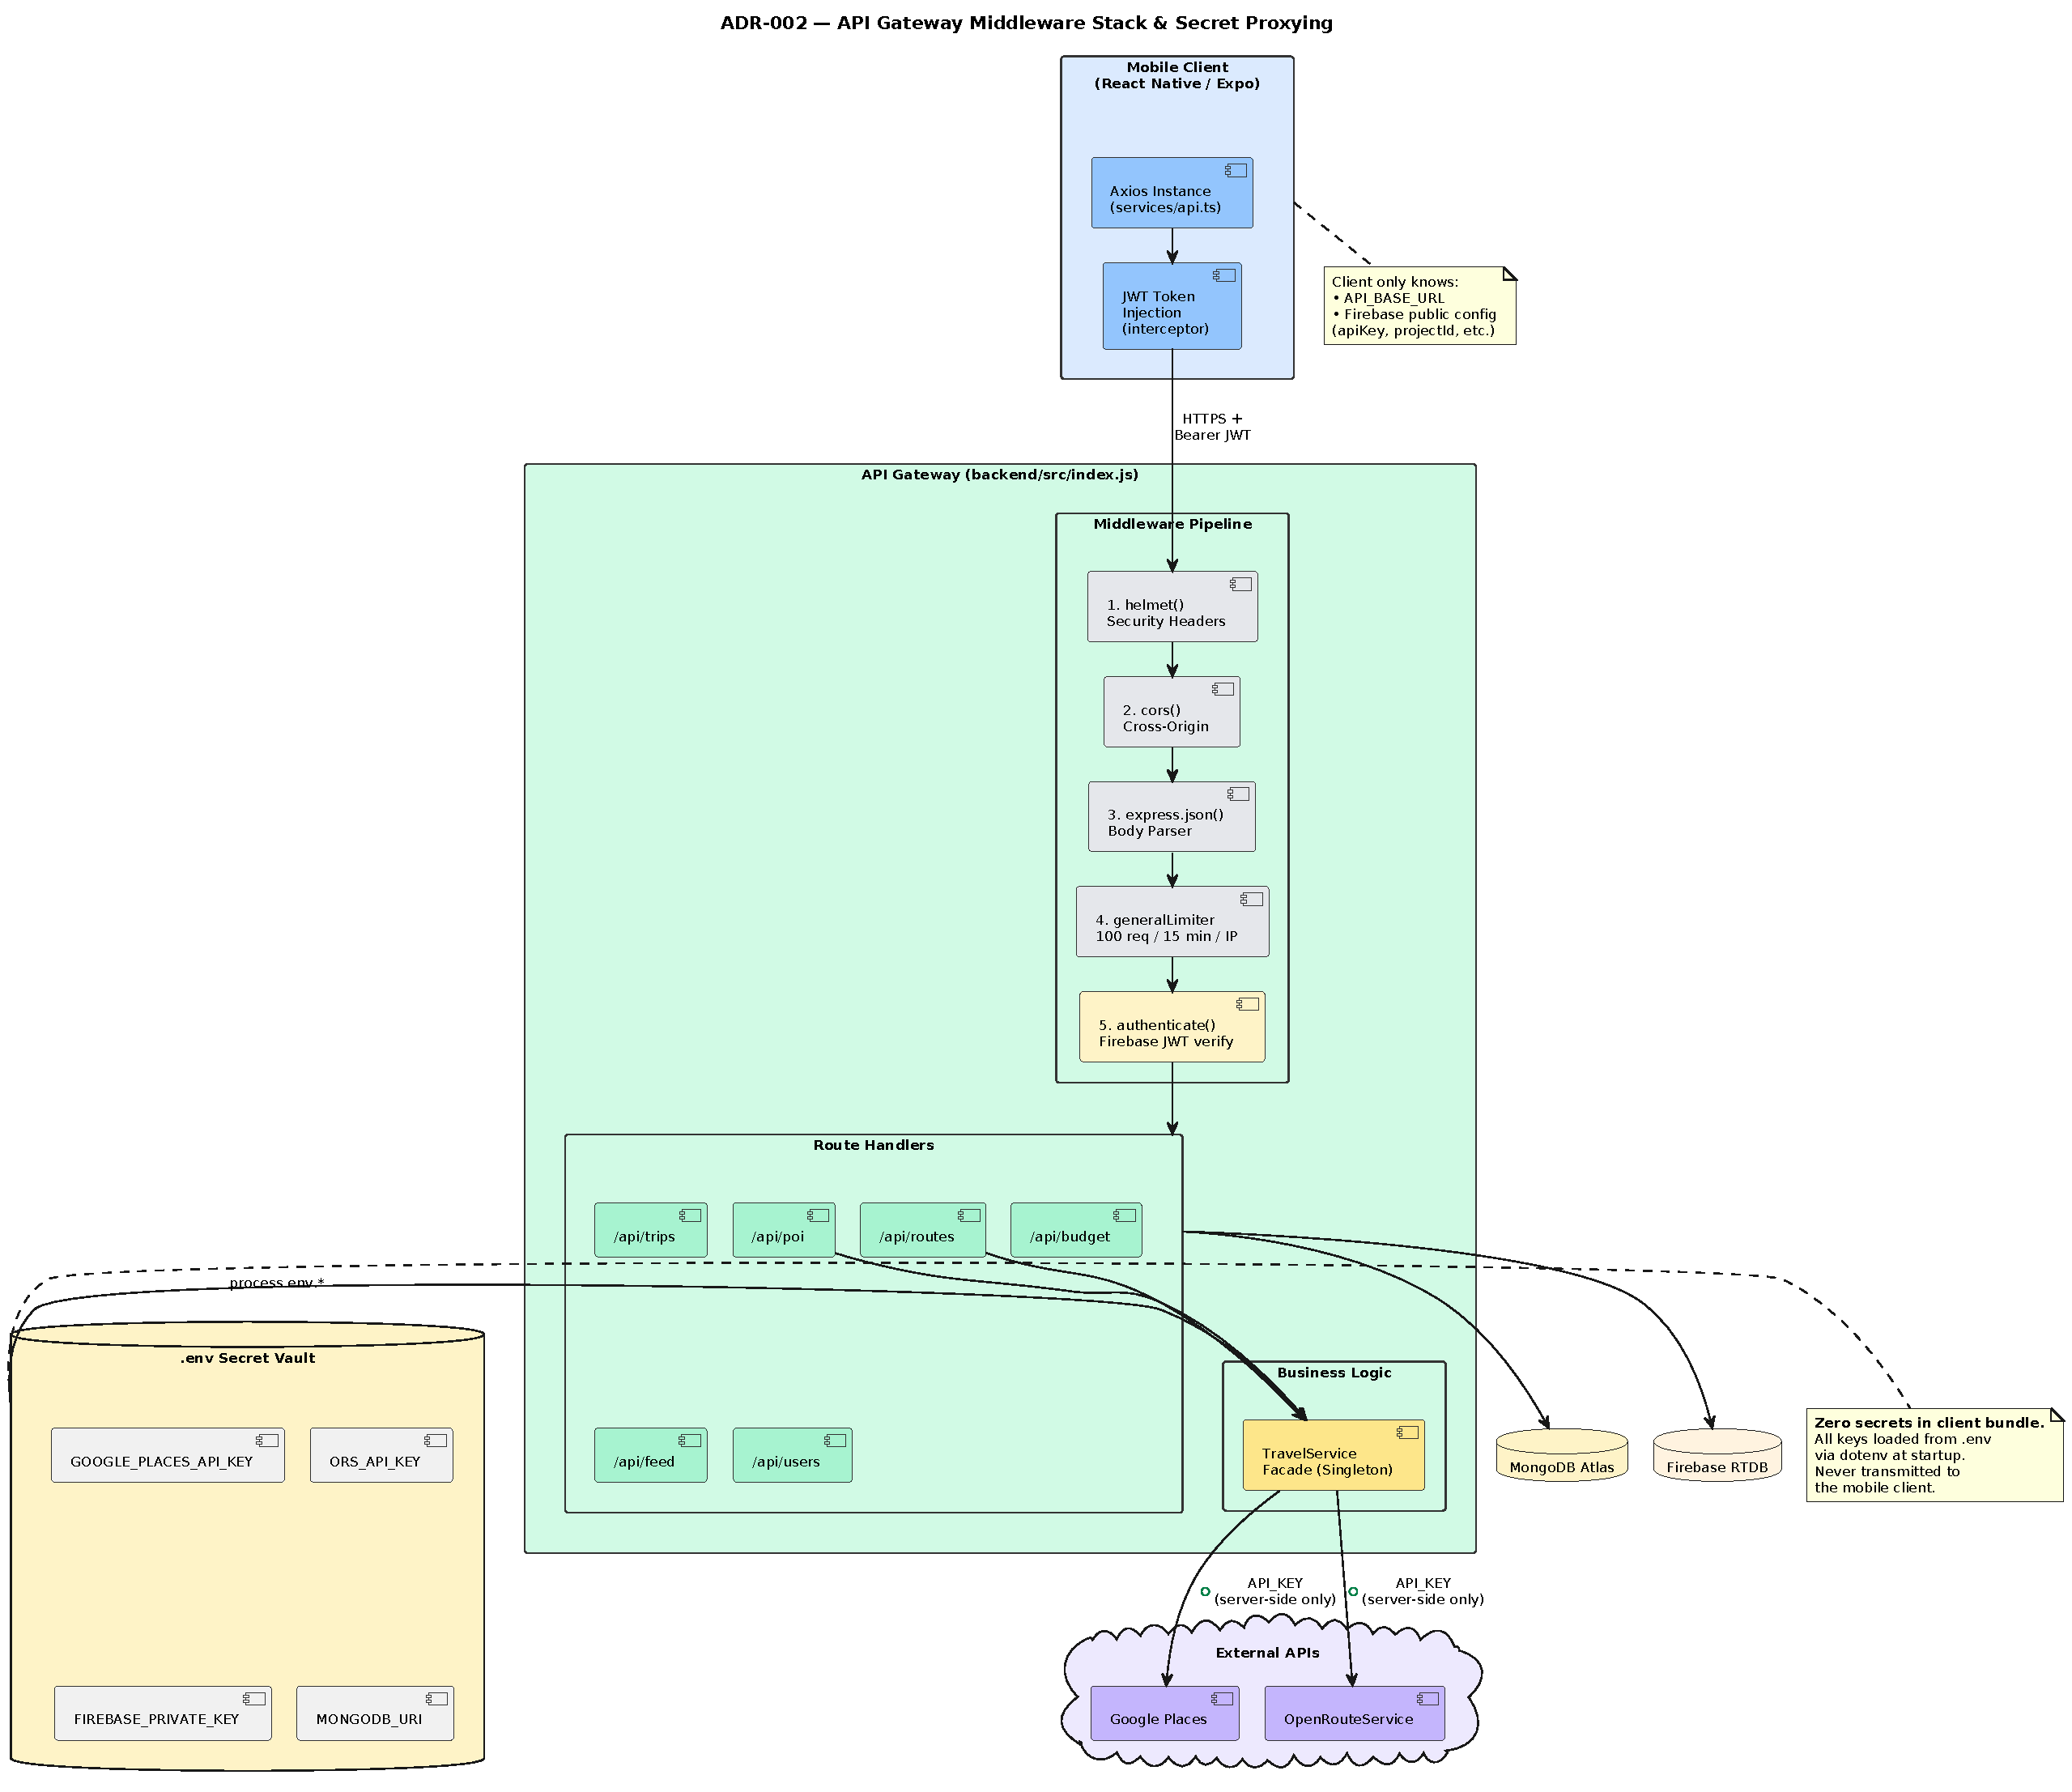
\includegraphics[width=\textwidth]{adr002_gateway_stack.pdf}
\caption{ADR-002 Component Diagram: API Gateway middleware pipeline and secret proxying flow. Requests from the mobile client pass through five middleware stages (helmet $\to$ cors $\to$ body parser $\to$ rate limiter $\to$ JWT auth) before reaching route handlers. External API keys are loaded from \code{.env} and injected by the TravelService Facade --- the mobile client never sees them.}
\label{fig:adr002-gateway}
\end{figure}

% -----------------------------------------------------------
\subsection{ADR-003: Implement the Facade + Strategy Pattern for Multi-provider POI Access}
% -----------------------------------------------------------

\begin{tcolorbox}[adrbox]

\textbf{\large ADR-003: TravelService Facade with Interchangeable Adapter Strategies}

\vspace{0.6em}
\textbf{Context}

WanderMate's POI discovery and routing features require integration with multiple external APIs, each with different protocols, response formats, quota limits, and failure modes:

\begin{longtable}{L{2.5cm} L{3.0cm} L{2.8cm} L{2.8cm}}
\toprule
\rowcolor{tableheaderbg}
\thcell{Provider} & \thcell{Protocol} & \thcell{Free-tier Quota} & \thcell{Data Quality} \\
\midrule
Google Places & REST, JSON & 5,000 req/month & Rich (photos, ratings, hours, price levels) \\
\rowcolor{tablealtbg}
ORS (POI) & REST, GeoJSON & 2,000 req/day & Basic (name, category, coordinates) \\
ORS (Routing) & REST, GeoJSON & 2,000 req/day & Good (directions + VROOM optimization) \\
\rowcolor{tablealtbg}
Overpass & Overpass QL & Unlimited (mirrors) & Varies (raw OSM data) \\
\bottomrule
\end{longtable}

Two architectural approaches were considered:
\begin{enumerate}
  \item \textbf{Direct API calls in routes:} Each Express route handler directly calls whichever provider it needs, with inline response normalisation, caching, and fallback logic.
  \item \textbf{Facade + Strategy:} A single \code{TravelService} class encapsulates all provider logic behind a unified interface, delegating to interchangeable adapter classes.
\end{enumerate}

Without a unifying layer, adding or swapping a provider would require modifying every route handler that uses POI data --- violating NFR-15 (provider swappability requires changes only in the adapter and Facade).

\vspace{0.6em}
\textbf{Decision}

We will implement a \code{TravelService} class (\code{services/travelService.js}) that combines the \textbf{Facade} and \textbf{Strategy} patterns:

\begin{enumerate}
  \item \textbf{Facade interface:} Six public methods --- \code{searchPOI()}, \code{searchByCategory()}, \code{getPlaceDetails()}, \code{getRoute()}, \code{optimizeRoute()}, \code{geocode()} --- abstract away all provider, caching, sorting, and geocoding logic.
  \item \textbf{Strategy adapters:} Three adapter classes, each wrapping a specific API behind a common normalised output:
    \begin{itemize}
      \item \code{PlacesAdapter} (\code{services/placesAdapter.js}) --- wraps Google Places (Text Search, Nearby Search, Find Place, Place Details). Supports 13 POI categories mapped to Google Places types. Normalises responses into the shared POI shape.
      \item \code{ORSAdapter} (\code{services/orsAdapter.js}) --- wraps ORS POI and routing endpoints. Category mappings use ORS category IDs (e.g., shopping: 500, medical: 460, finance: 430). Implements both simple routing (\code{/v2/directions}) and multi-stop optimization (\code{/optimization}).
      \item \code{OverpassAdapter} (\code{services/overpassAdapter.js}) --- implemented but currently disabled.
    \end{itemize}
  \item \textbf{Proximity sorting:} Both \code{searchPOI()} and \code{searchByCategory()} compute the Haversine great-circle distance between the map centre and each POI using \code{\_calculateDistance(lat1, lon1, lat2, lon2)}, sort results by ascending distance, and apply a relevancy cap (15 results for text queries, 20 for category queries).
  \item \textbf{Singleton:} A module-level instance (\code{let instance = null}) with a \code{getTravelService()} factory function ensures one instance is shared across all route modules.
  \item \textbf{Caching:} A single \code{node-cache} instance inside the Facade applies per-method TTLs: 30~minutes for searches, 24~hours for details, 1~hour for routes, using key patterns such as \code{poi:*}, \code{cat:*}, \code{details:*}, and \code{route:*}.
  \item \textbf{Fallback chain:} \code{searchPOI()} attempts Google Places first, catches failures, and falls through to ORS:
  \begin{verbatim}
    results = await this.places.searchPOI(query, lat, lng, radius)
                   .catch(err => { return []; });
    if (results.length === 0) {
        results = await this.ors.searchPOI(query, lat, lng, radius)
                     .catch(err => { return []; });
    }
  \end{verbatim}
\end{enumerate}

\vspace{0.6em}
\textbf{Status:} \adrstatus{Accepted}

\vspace{0.6em}
\textbf{Consequences}

\textbf{Positive:}
\begin{itemize}
  \item \textbf{Provider independence:} Route handlers in \code{routes/poi.js} call \code{travelService.searchPOI()} (line~18) without knowing which provider responded. Adding Mapbox or HERE requires only a new adapter class and a registration line in the \code{TravelService} constructor.
  \item \textbf{Validated swappability:} The \code{OverpassAdapter} was disabled by commenting out its import in \code{travelService.js} --- zero changes to routes, stores, or UI components. This validates NFR-15.
  \item \textbf{Centralized caching:} One \code{node-cache} instance serves all providers; no duplicate cache logic. Cache key generation follows stable prefixed keys (for example: \code{poi:...}, \code{cat:...}, \code{details:...}, \code{route:...}).
  \item \textbf{Graceful degradation:} The fallback chain (Google $\to$ ORS $\to$ empty) is invisible to consumers, satisfying NFR-08.
\end{itemize}

\textbf{Negative:}
\begin{itemize}
  \item An additional layer of abstraction increases code navigation complexity; developers must trace calls through the Facade to reach adapter implementations.
  \item The normalised POI interface is a least-common-denominator: rich Google Places data (photos, opening hours, price levels) is flattened alongside ORS's basic data, potentially underutilising provider-specific features.
  \item The fallback chain introduces latency when the primary provider fails. Two sequential API calls (Google $\to$ ORS) are made before returning results, though caching mitigates this for repeated queries.
\end{itemize}

\end{tcolorbox}

\begin{figure}[H]
\centering
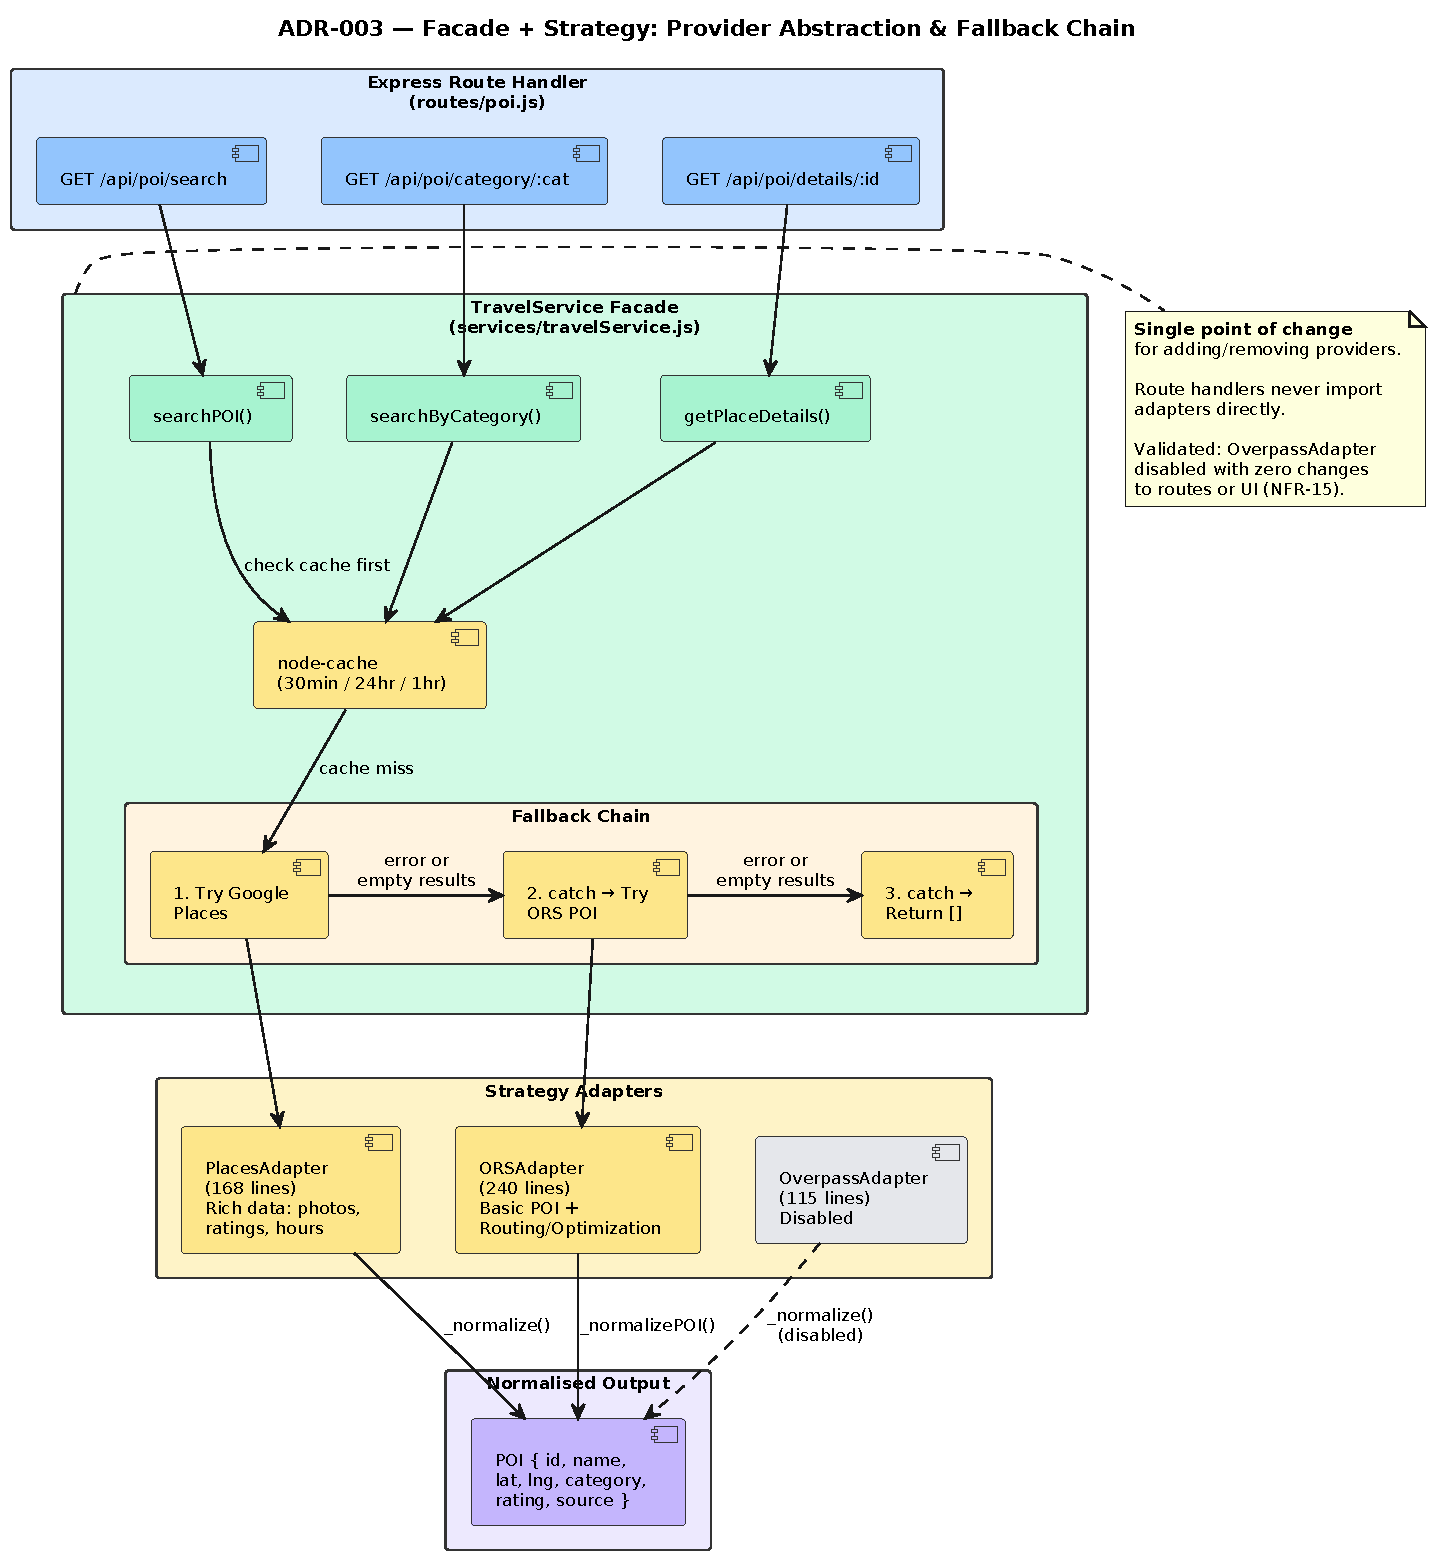
\includegraphics[width=0.90\textwidth]{adr003_facade_decision.pdf}
\caption{ADR-003 Component Diagram: the TravelService Facade receives calls from route handlers, checks the \code{node-cache}, and dispatches to the fallback chain (Google Places $\to$ ORS $\to$ empty array). All adapters normalise responses to a common POI interface. The OverpassAdapter is implemented but currently disabled.}
\label{fig:adr003-facade}
\end{figure}

% -----------------------------------------------------------
\subsection{ADR-004: Adopt an Offline-First Architecture with AsyncStorage and a Persistent Sync Queue}
% -----------------------------------------------------------

\begin{tcolorbox}[adrbox]

\textbf{\large ADR-004: Offline-First Client with AsyncStorage Cache and SyncQueue}

\vspace{0.6em}
\textbf{Context}

Travel applications must function in environments with unreliable or no connectivity: airports during boarding, remote hiking trails, underground metro stations, and international roaming situations where data is expensive. WanderMate users must be able to:

\begin{itemize}
  \item View their itineraries, trip details, and budget data while offline (\reqid{FR-03}, \reqid{NFR-07}).
  \item Edit trips (add/remove stops, modify notes) while offline, with changes synchronised when connectivity is restored.
  \item Not lose any data due to transient network failures.
\end{itemize}

Two approaches were considered:
\begin{enumerate}
  \item \textbf{Online-required:} All operations require network connectivity. Offline access shows a ``No connection'' error screen.
  \item \textbf{Offline-first:} All reads are served from a local cache first. Writes are queued locally and replayed to the server on reconnect.
\end{enumerate}

\vspace{0.6em}
\textbf{Decision}

We will implement an \textbf{offline-first architecture} using two modules in \code{frontend/services/syncQueue.ts}:

\begin{enumerate}
  \item \textbf{\code{localCache}} --- a key-value cache backed by AsyncStorage with configurable TTL:
  \begin{verbatim}
    export const localCache = {
      async get(key, maxAgeMs = 3600000) { /* 1 hour default */ },
      async set(key, data) { /* stores {data, cachedAt} */ },
      async remove(key) { /* removes entry */ }
    };
  \end{verbatim}
  Every Zustand store method (e.g., \code{tripStore.fetchTrips()}) follows a try/catch pattern: attempt the API call, and on failure, read from \code{localCache} with infinite TTL (\code{Infinity}):
  \begin{verbatim}
    try { response = await api.get('/trips'); }
    catch {
        const cached = await localCache.get('trips', Infinity);
        if (cached) set({ trips: cached });
    }
  \end{verbatim}

  \item \textbf{\code{syncQueue}} --- a persistent mutation queue backed by AsyncStorage:
  \begin{verbatim}
    export const syncQueue = {
      async add(operation) {
        const queue = await this.getAll();
        queue.push({ ...operation, timestamp: Date.now(), id });
        await AsyncStorage.setItem(QUEUE_KEY, JSON.stringify(queue));
      },
      async flush() {
        const queue = await this.getAll();
        for (const op of queue.sort((a,b) => a.timestamp - b.timestamp)) {
          // replay POST/PUT/DELETE via api client
        }
      }
    };
  \end{verbatim}
  When selected write operations fail (network error), the store catches the exception and enqueues the mutation. The queue is flushed on reconnect via the Profile screen's ``Sync Offline Changes'' button, replaying operations in timestamp order.
\end{enumerate}

\vspace{0.6em}
\textbf{Status:} \adrstatus{Accepted}

\vspace{0.6em}
\textbf{Consequences}

\textbf{Positive:}
\begin{itemize}
  \item \textbf{Zero-downtime reads:} Users can browse all previously loaded trips, stops, and budget data without connectivity. The \code{localCache} serves stale data with infinite TTL, preferable to a blank screen.
  \item \textbf{No data loss:} Write operations are persisted to AsyncStorage immediately. Even if the app is closed and reopened, the queue survives and can be flushed.
  \item \textbf{Simple conflict resolution:} Mutations are replayed in timestamp order (FIFO). Combined with the server-side last-write-wins semantics (\code{updatedAt} timestamps), this provides eventual consistency without complex merge logic.
  \item \textbf{AsyncStorage is already a dependency:} Used for Firebase auth persistence (\code{getReactNativePersistence(AsyncStorage)} in \code{config/firebase.ts}), so no additional dependency is introduced.
\end{itemize}

\textbf{Negative:}
\begin{itemize}
  \item \textbf{Stale data risk:} Offline users see the last-cached state, which may diverge significantly from the current server state if collaborators have been making changes.
  \item \textbf{Queue conflicts:} If two offline users make conflicting edits (e.g., both remove the same stop), the second flush will encounter a 404 or produce an inconsistent state. Last-write-wins resolves this but may silently discard one user's changes.
  \item \textbf{Sync trigger --- automatic and manual:} The queue is flushed automatically on every app launch and whenever the app transitions to the \code{active} state (via an \code{AppState} listener wired in \code{app/\_layout.tsx}). A manual ``Sync Offline Changes'' button on the Profile screen provides an additional on-demand trigger. The automatic flush covers the common reconnection scenario; the manual button serves as a fallback for edge cases (e.g., the user stays in-app while connectivity is restored).
  \item \textbf{Queue growth during extended offline periods:} If a user remains offline for an extended period while making many edits, the \code{syncQueue} in AsyncStorage can grow unboundedly. Large queues increase both the flush duration and the probability of conflicts. A future improvement could cap the queue size or batch related mutations (e.g., multiple edits to the same stop) into a single consolidated operation.
  \item \textbf{Deleted resource handling:} If a collaborator deletes a trip or stop while another user is offline, queued mutations targeting that resource will receive 404 responses during flush. The current \code{flush()} implementation keeps failed operations for future retries; robust handling could classify permanent errors (404/410) and discard stale operations automatically.
  \item \textbf{AsyncStorage performance:} Large trip documents serialised to JSON may incur noticeable read/write latency; AsyncStorage is not designed for high-frequency updates.
\end{itemize}

\end{tcolorbox}

\begin{figure}[H]
\centering
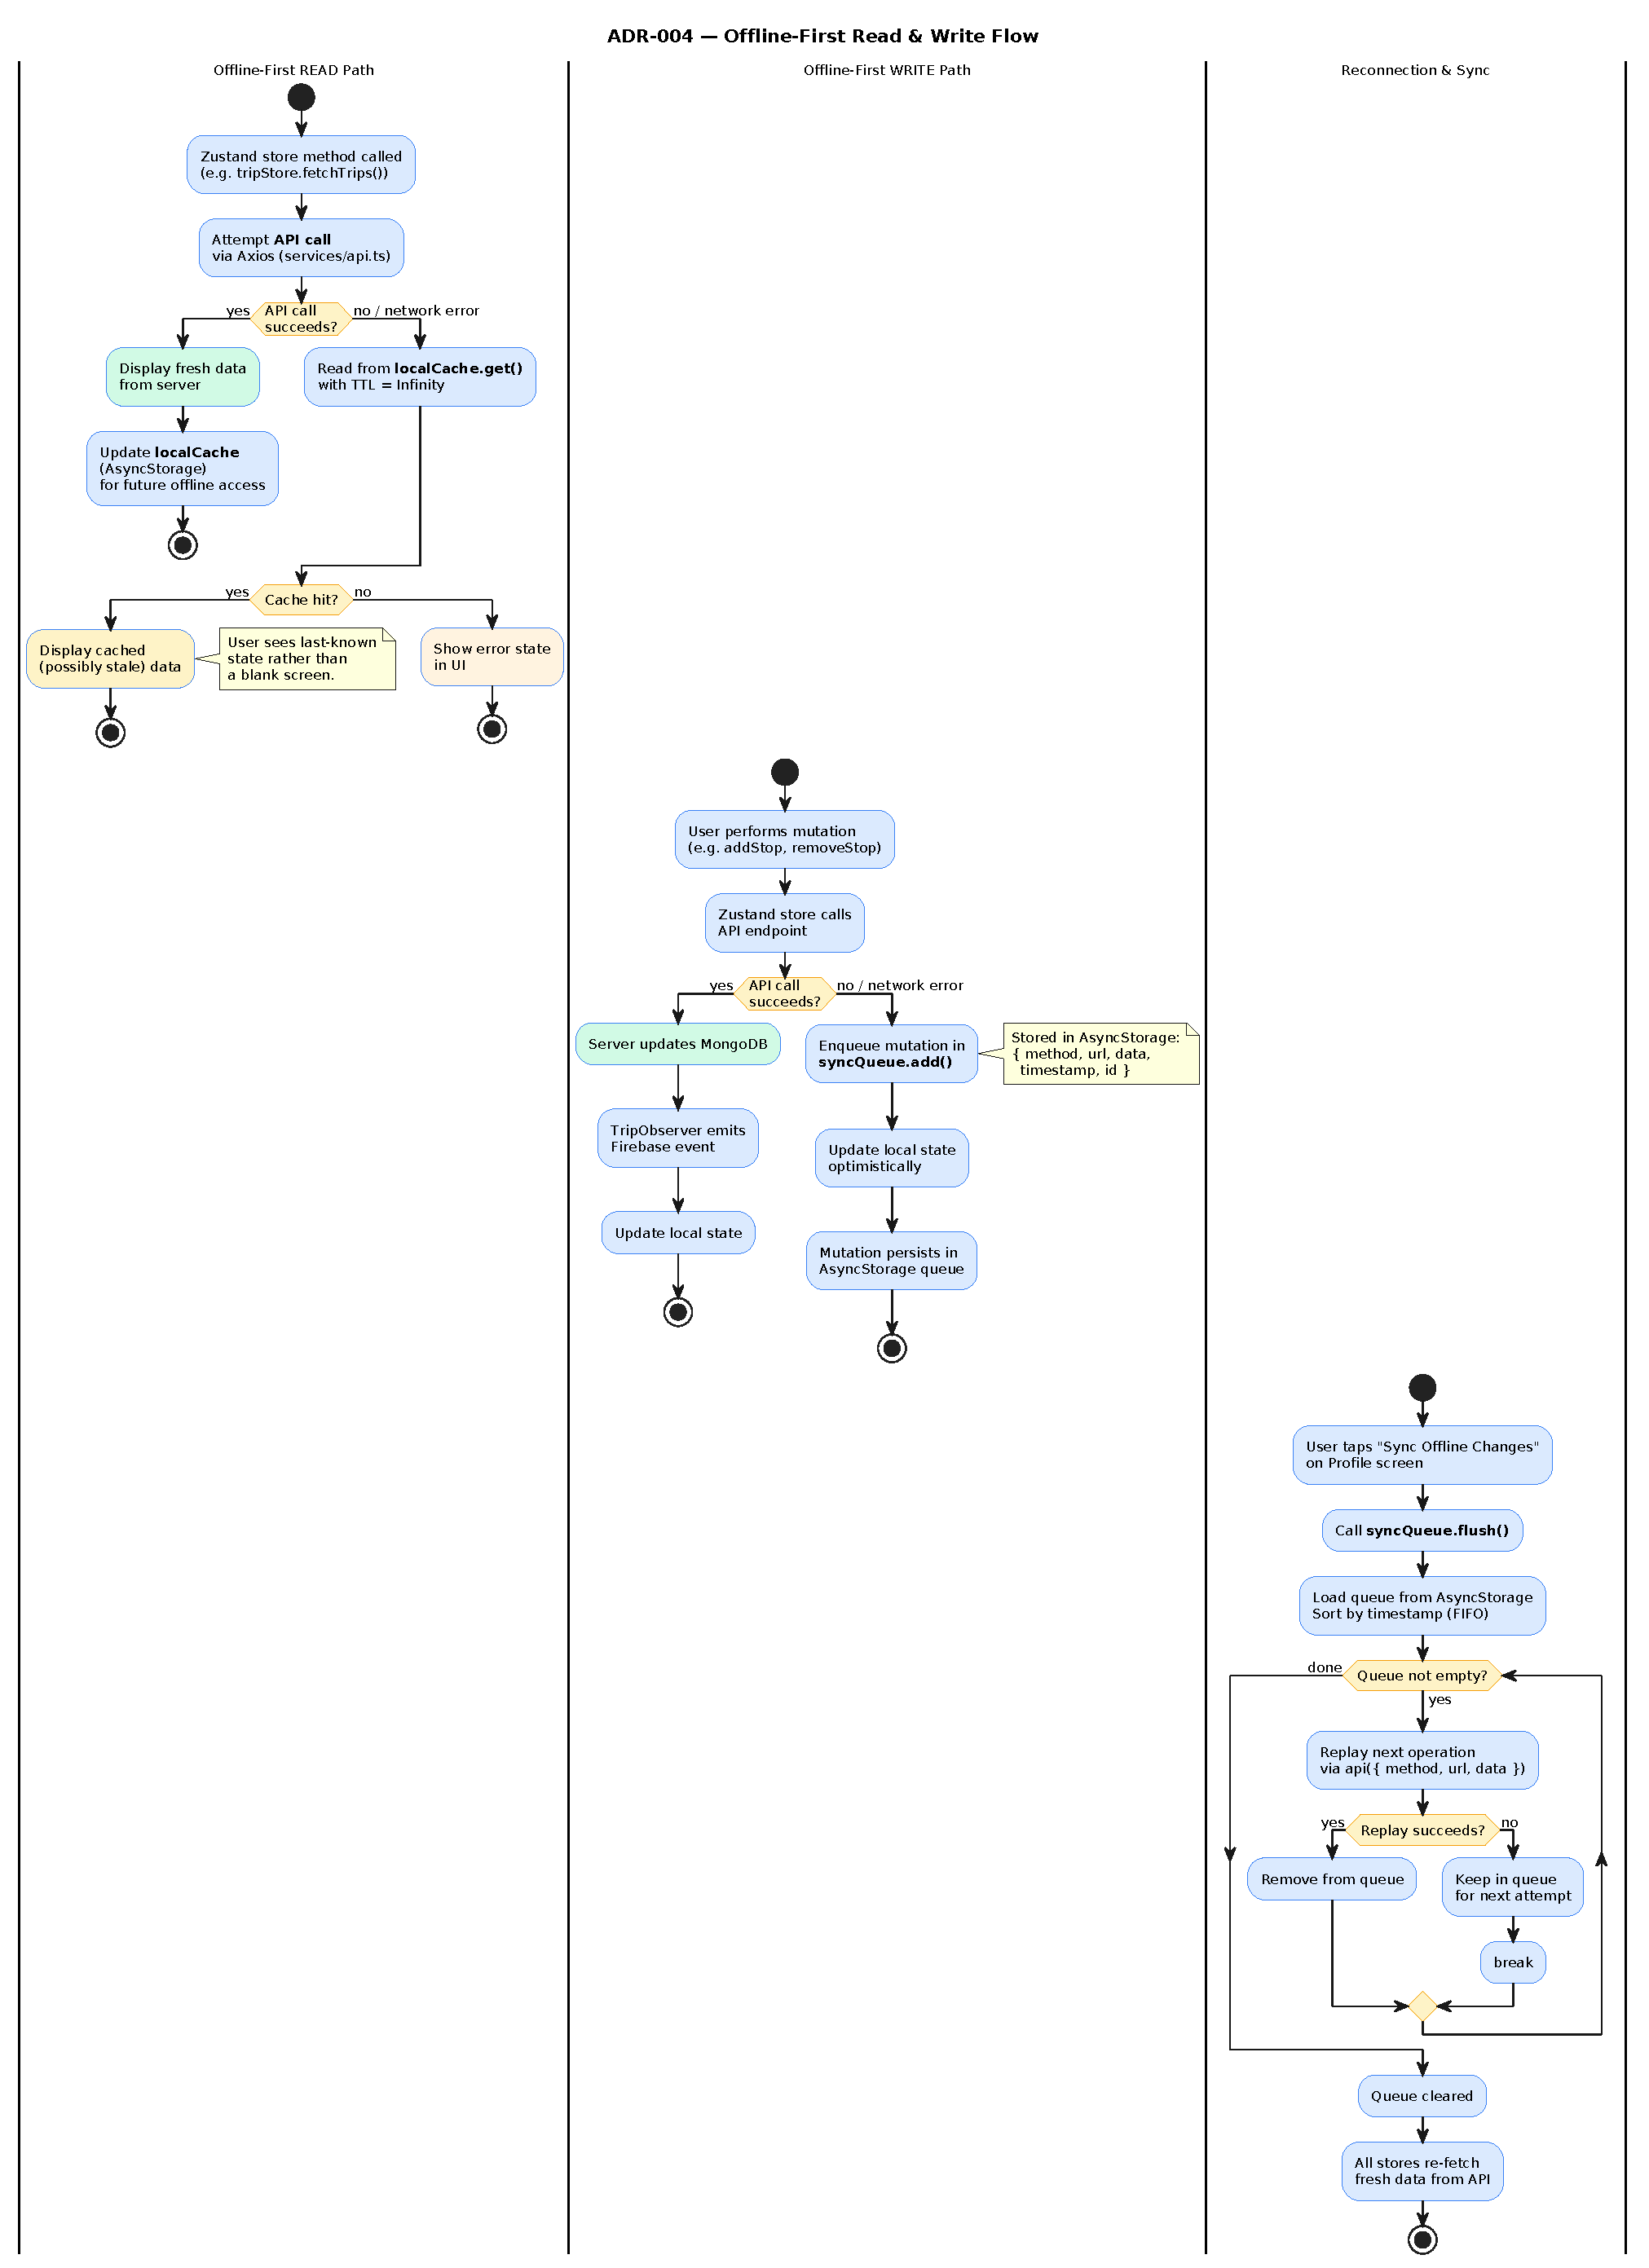
\includegraphics[width=0.85\textwidth]{adr004_offline_flow.pdf}
\caption{ADR-004 Activity Diagram: offline-first read and write flows. \textbf{Read path:} API call attempted $\to$ on failure, \code{localCache} serves stale data with TTL = Infinity. \textbf{Write path:} API call attempted $\to$ on failure, mutation enqueued via \code{syncQueue.add()} and persisted in AsyncStorage. \textbf{Sync path:} on reconnect, \code{syncQueue.flush()} replays operations in timestamp order.}
\label{fig:adr004-offline}
\end{figure}

% ============================================================
\section{ADR Summary and Cross-references}
% ============================================================

The following table summarises all four ADRs and maps them to the stakeholder concerns and NFRs they address:

\begin{longtable}{C{1.2cm} L{3.5cm} C{1.5cm} L{2.5cm} L{4.0cm}}
\toprule
\rowcolor{tableheaderbg}
\thcell{ADR} & \thcell{Decision} & \thcell{Status} & \thcell{Concerns} & \thcell{NFRs Addressed} \\
\midrule
\endhead
\bottomrule
\endfoot

001 & Firebase RTDB as collaboration sync channel; MongoDB as source of truth & \adrstatus{Accepted} & C7 (Real-time), C3 (Offline) & NFR-03 (sync $<$500ms), FR-20/21 (collaboration) \\

\rowcolor{tablealtbg}
002 & API Gateway with secret proxying & \adrstatus{Accepted} & C2 (Security), C6 (Quota) & NFR-11 (no client secrets), NFR-06 (quota), NFR-10 (HTTPS) \\

003 & Facade + Strategy for multi-provider POI & \adrstatus{Accepted} & C4 (Modifiability), C6 (Quota) & NFR-15 (swappability), NFR-08 (fallback), NFR-06 (caching) \\

\rowcolor{tablealtbg}
004 & Offline-first architecture with AsyncStorage & \adrstatus{Accepted} & C3 (Offline), C1 (Usability) & NFR-07 (offline availability), FR-03 (local persistence) \\

\end{longtable}

\begin{tcolorbox}[notebox]
  \textbf{Inter-ADR dependencies.} ADR-001 (Firebase as collaboration sync channel) depends on ADR-002 (API Gateway) because the gateway is the component that writes synchronization updates to Firebase after persisting to MongoDB. ADR-003 (Facade pattern) is implemented within the gateway defined by ADR-002. ADR-004 (offline-first) complements ADR-001 by providing a client-side persistence layer that bridges connectivity gaps.
\end{tcolorbox}

% ============================================================
\section{Conclusion}
% ============================================================

This document has presented the Architecture Framework for WanderMate following two complementary approaches:

\textbf{IEEE 42010 Stakeholder Analysis} identified five stakeholder classes (End Users, Development Team, Project Supervisor, System Administrator, API Providers) and seven concrete concerns spanning usability, security, offline availability, modifiability, deployment, quota compliance, and real-time collaboration. Four architecture viewpoints (Functional, Information, Deployment, Development) were defined with concrete views grounded in the codebase, providing full traceability from stakeholder concerns through viewpoints to specific code artefacts and requirements.

\textbf{Nygard ADR documentation} captured four major design decisions:
\begin{enumerate}
  \item Using Firebase RTDB as a collaboration synchronization channel while MongoDB remains the authoritative data store (ADR-001).
  \item Adopting the API Gateway pattern to protect secrets and centralise policy enforcement (ADR-002).
  \item Implementing the Facade + Strategy pattern for multi-provider POI access with caching and fallback (ADR-003).
  \item Building an offline-first client with AsyncStorage-backed caching and a persistent sync queue (ADR-004).
\end{enumerate}

Each decision was documented with its full context, the alternatives considered, the chosen approach with supporting code evidence, and an honest assessment of both positive and negative consequences. Together, these decisions form a coherent architectural strategy that balances the competing forces of real-time collaboration, offline availability, API quota constraints, security, and long-term maintainability.

\end{document}
